\chapter{Umsetzung des Prototyps}
Nachdem in Kapitel \ref{sec:concept} die Konzeption der Anwendung vorgestellt wurde kann, kann nun die Umsetzung der Anwendungen erfolgen.

Zunächst wird dabei auf die Ausgangssituation aus dem vorangegangenem Projekt vorgestellt. Im Anschluss erfolgt eine Auflistung der verwendeten Technologien. Danach erfolgt die Vorstellung der Anwendungen, sowie die Herausforderungen und Probleme in der Umsetzung

\section{Ausgangssituation}
In der vorausgehenden Arbeit wurde ein Art \ac{MVP} der Spielidee umgesetzt welche aus 3 Hauptanwendungen bestand. Es gibt eine Unity-Anwendung, in welcher das Spielgeschehen des \say{Players} umgesetzt wurde. Das Spielgeschehen der \say{Watcher}-Anwendung wurde über eine Vue3-Webseite realisiert. Für die Kommunikation der beiden Anwendungen untereinander wurde auf der Basis eines \say{Express.js} Node-Servers ein WebSocket-Server entwickelt. Der Node-WebSocket-Server kommuniziert zusätzlich mit einer MongoDB Datenbank, in welcher die Fortschritte der einzelnen Sessions gespeichert werden.

Die Anwendungen des \say{Players} und des \say{Watchers} sind in dieser Konstellation jeweils Anzeigende und auf die Eingaben des Nutzers reagierende Komponenten im gesamten System. Sie geben eine Rückmeldung an den Server, der die Daten zur Laufzeit abspeichert und persistent in einer Datenbank speichern kann.

\subsection{Aufbau der Ausgangssituation}

Im Softwaredesign wird dabei von einem \ac{MVC} Design-Pattern gesprochen (vgl. \cite{GlossarWiki:Reenskaug:1979a}). 
Das Model definiert, welche Daten die App enthalten soll. Ändert sich der Zustand dieser Daten, informiert das Modell die einzelnen Views, damit die Ansicht der Daten entsprechend aktualisiert werden können. Außerdem wird manchmal auch der Controller über Änderungen informiert. Die View definiert wie die Daten angezeigt werden sollen. Der Controller verarbeitet die reinkommenden Änderungen aus den Views, die die Nutzer getätigt haben, und gibt diese an das Model oder die Views direkt weiter (vgl. \cite{noauthor_mvc_2023}); (vgl. Abbildung \ref{fig:mvc-diagramm}).

\begin{figure}[ht]
\centering
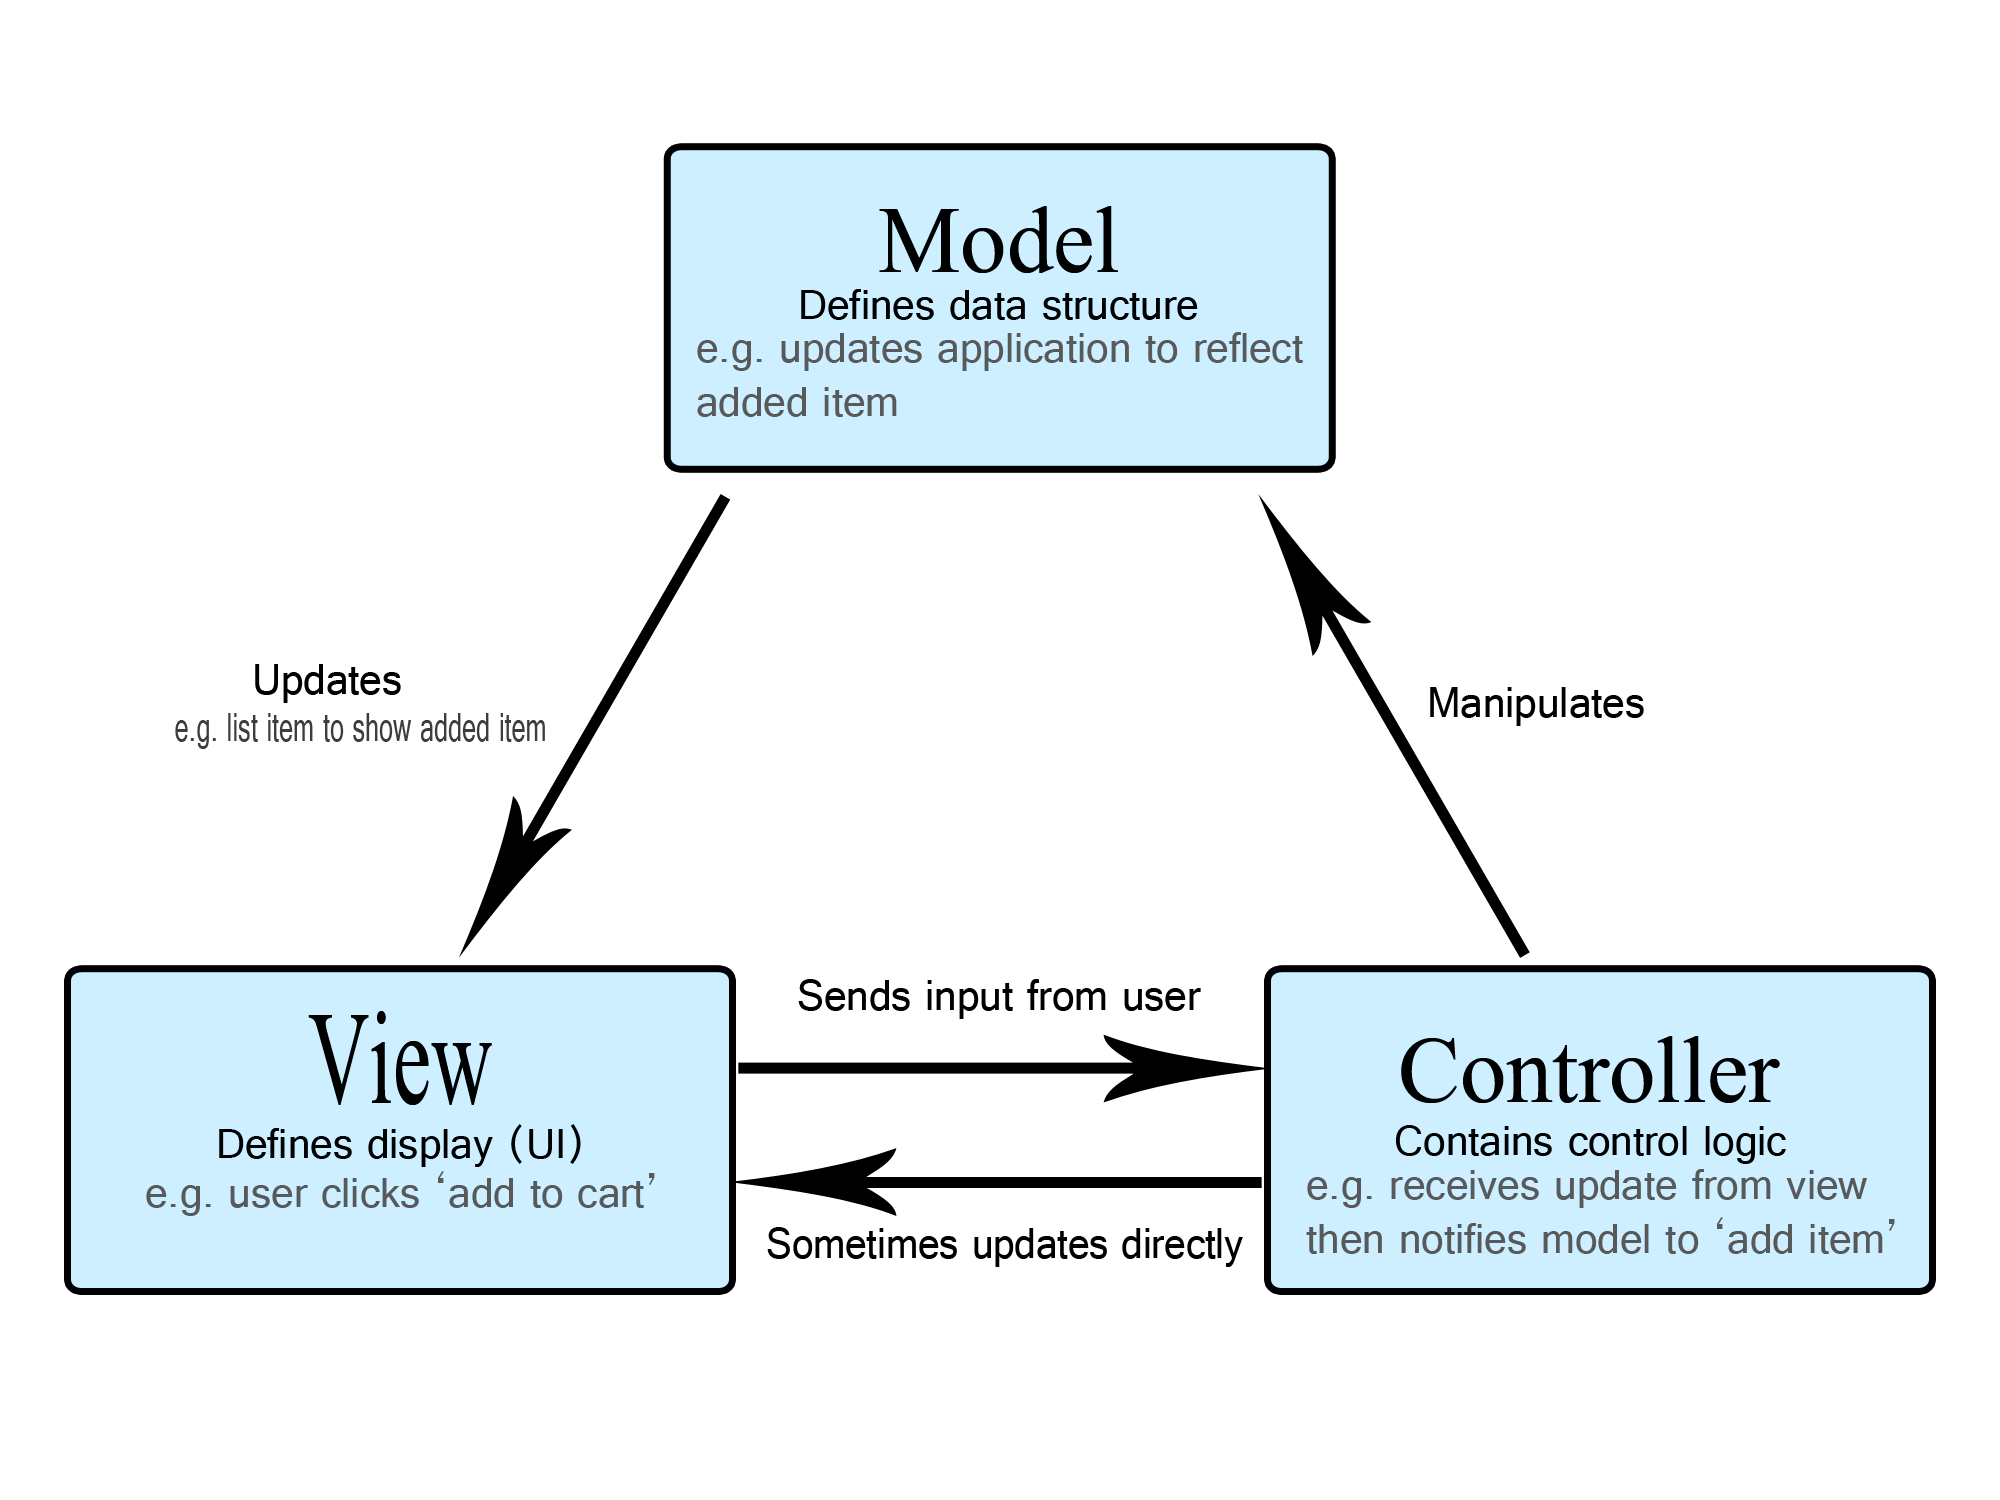
\includegraphics[width=1\linewidth]{content/pictures/mvc-architecture.png}
\caption{\ac{MVC} Beispiel-Diagramm (Quelle: \cite{noauthor_mvc_2023})}
\label{fig:mvc-diagramm}
\end{figure}

Die MongoDB Datenbank und Klassen innerhalb des WebSocket-Servers nehmen die Rolle des Model ein, die einzelnen WebSocket-Nachricht Endpunkte übernehmen die Aufgaben des Controllers und die Anwendung des \say{Watchers} und des \say{Players} sind die Views der Architektur.

\subsection{Beitreten einer Session}

\begin{figure}[ht]
\centering
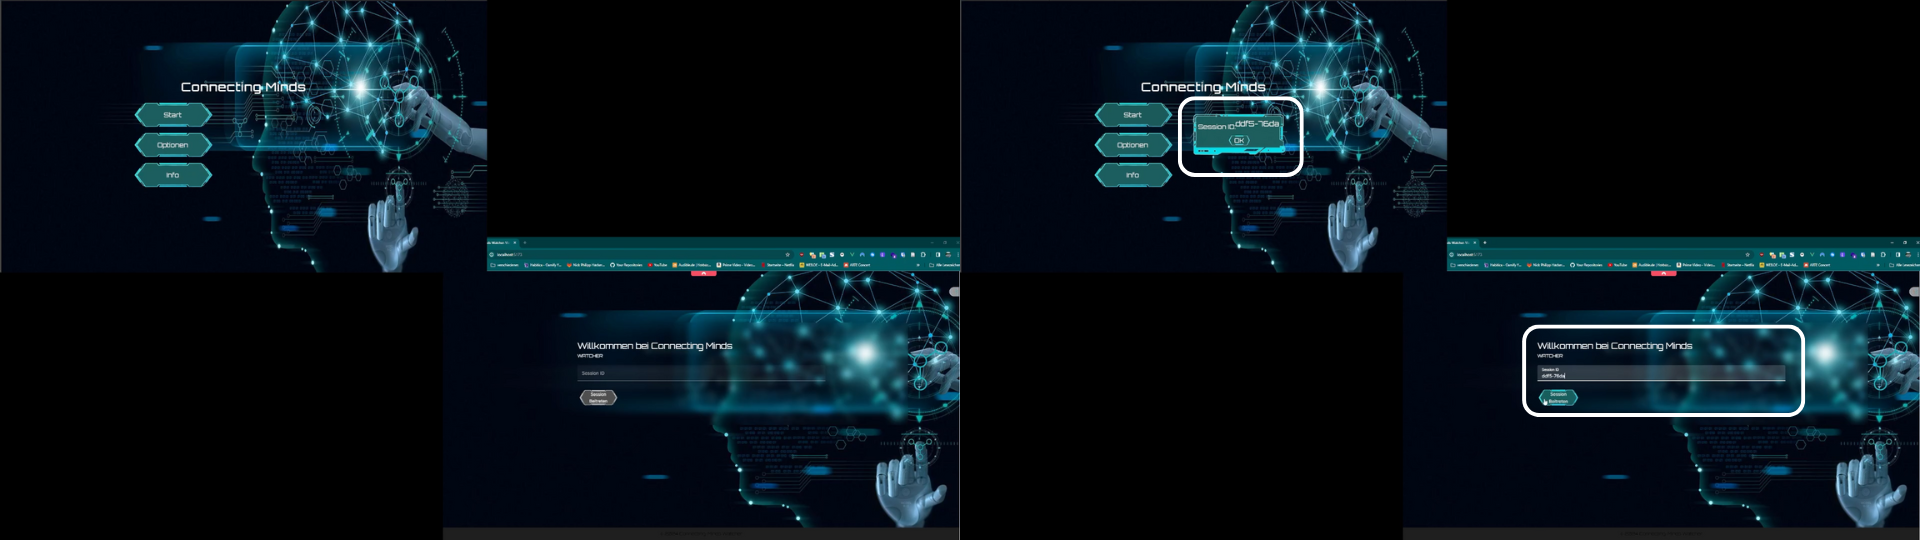
\includegraphics[width=1\linewidth]{content/pictures/Login_Login_by_ID.png}
\caption{Startbildschirme der Player und Watcher Anwendung (Quelle: eigene Darstellung)}
\label{fig:old-logins}
\end{figure}

Abbildung \ref{fig:old-logins} zeigt den bereits im alten Prototyp entwickelten Startbildschirm über welchen der Player eine neue Session starten (linkes Bild, links oben) und der Watcher dieser beitreten kann (linkes Bild, rechts unten). Sobald der Player eine Session erstellt hat, erhält er vom WebSocket-Server eine Rückmeldung mit der erstellten Session-ID (rechtes Bild, links oben) welches er dem Watcher mitteilen muss, damit dieser ihr beitreten kann (rechts Bild, rechts unten).

\subsection{Einführung in die Anwendungen}

\begin{figure}[ht]
\centering
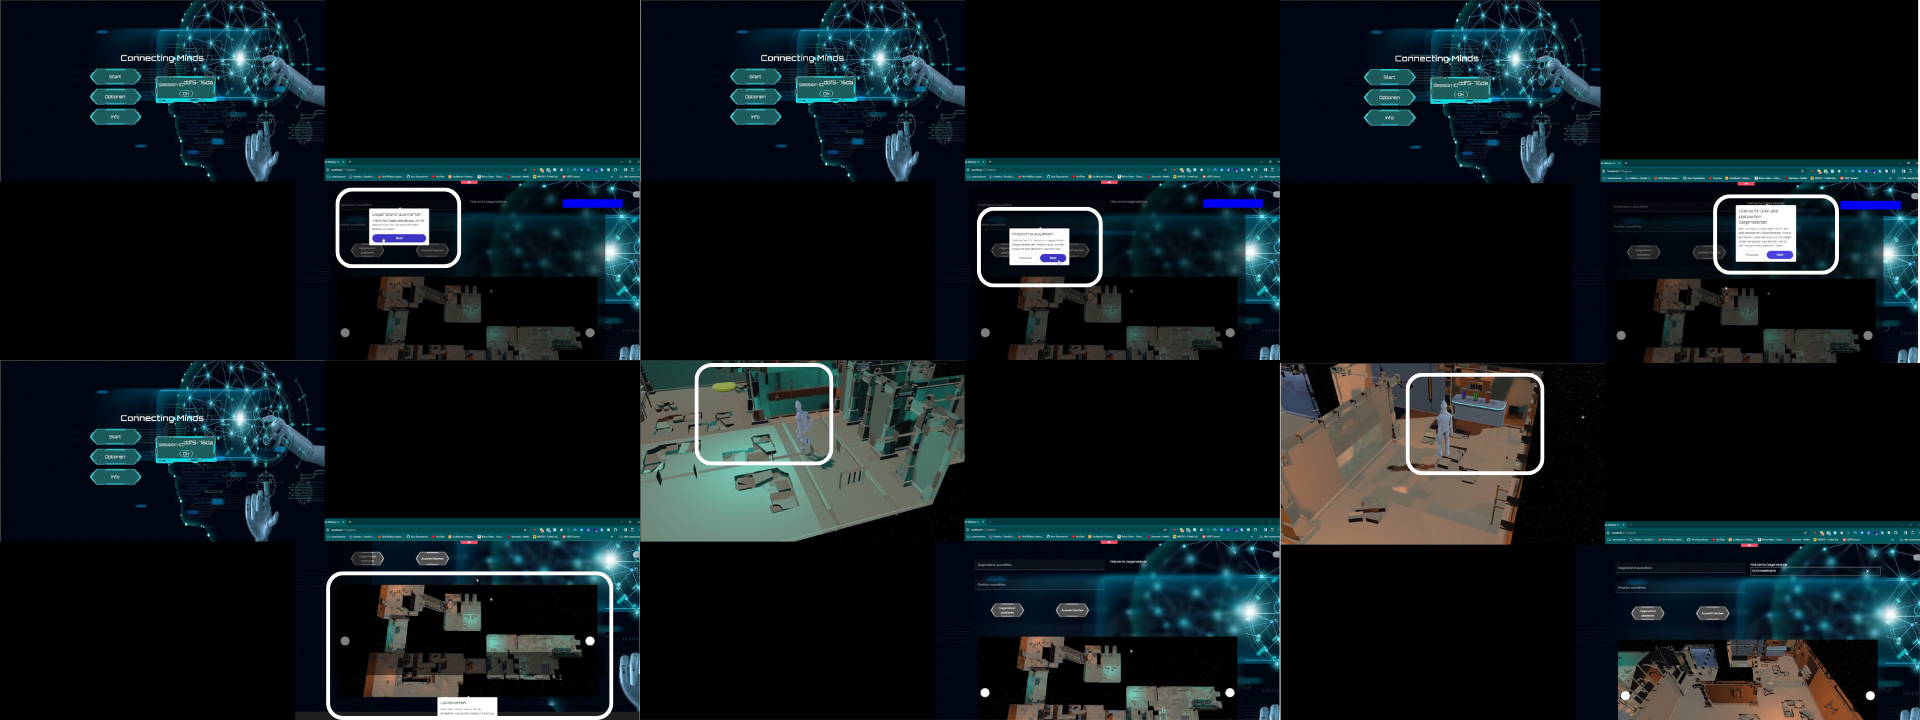
\includegraphics[width=1\linewidth]{content/pictures/Introduction.png}
\caption{Einführung in die Anwendung des Players und Watchers (Quelle: eigene Darstellung)}
\label{fig:old-introductions}
\end{figure}

Abbildung \ref{fig:old-introductions} zeigt die Einführung der beiden Anwendungen in die Spielwelt. Zum Start erhielt der Watcher einzelne Tooltips, mit Erklärungen zu den Grundfunktionen seiner Anwendung (erstes bis drittes Bild in der ersten Zeile und linkes Bild in der zweiten Zeile; jeweils in weiß umrandet im rechten Bildelement). Seine Anwendung enthalten zwei Dropdown-Menüs, über die Gegenstände und Positionen ausgewählt werden können, (erste Zeile, Bilder links und und in der Mitte) eine Liste mit allen platzierten Gegenstände (erste Zeile rechts Bild), die jeweils einzeln entfernt werden können und eine Top-Down-Ansicht der Spielwelt, in der sich der Player befindet (zweite Zeile, linkes Bild). 

Der Player steuert seinen Avatar über eine Touch-druck auf die Spielwelt (zweite Reihe mittlere Bild, linkes Bildelement). Außerdem kann er über vertikale Swipes die Höher der Kamera zum Avatar verändern und dadurch in einem gewissen Rahmen die Ansicht verändern.

Um in der Spielwelt an das Ziel zu gelangen, müssen der Player und Watcher zusammenarbeiten und Hindernisse in der Spielwelt beseitigen. Im linken Bild in der zweiten Zeile im weiß umrandeten wird ein solches Rätselelement dargestellt, welches gelöst werden muss.
\subsection{Lösen von Rätseln}
Wie wurden im alten Prototyp die einzelnen Rätsel gelöst und durch wen erfolgte dies?

\begin{figure}[ht]
\centering
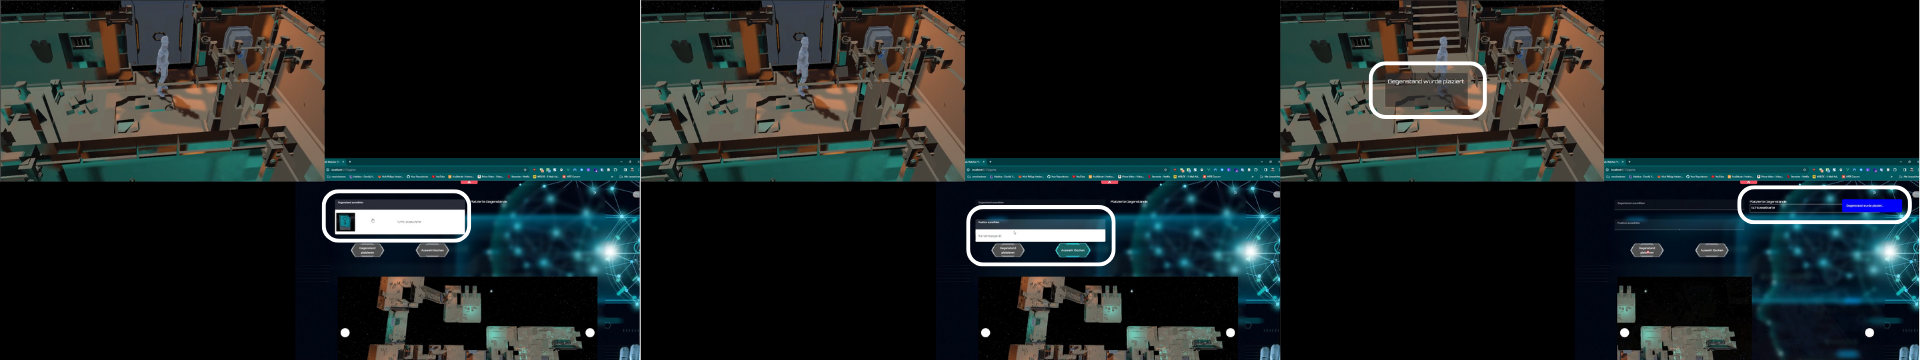
\includegraphics[width=1\linewidth]{content/pictures/HowToSolve.png}
\caption{Vorgang des Lösens von Rätseln (Quelle: eigene Darstellung)}
\label{fig:old-solving-riddle}
\end{figure}

Der Watcher war dafür verantwortlich, dass Gegenstände auf ihre richtigen Zielpositionen platziert wurden. Sobald der Player auf eine Absperrung in der Spielwelt stieß, musste er beschreiben was er sah um dem Watcher einen Hinweis darauf zu geben, welche Gegenstände platziert werden müssen und auf welche Positionen diese gehören. Zunächst wählt der Watcher über das Gegenstände-Dropdown einen entsprechenden Gegenstand aus (linkes Bild, rechtes Bildelement). Anschließend wählt er eine vorgegebene Position aus, die im derzeitig aktiven Abschnitt der Spielwelt hinzugekommen ist (mittlere Bild, rechts Bildelement). Über den Button \say{Gegenstand platzieren} (linker Button) wird der Gegenstand in die Spielwelt des Players platziert. Sowohl der Player als auch der Watcher erhalten vom System eine Benachrichtigung, dass der Gegenstand platziert wurde (rechts Bild, beide weißen Umrandungen). Auf der rechten Seite der Watcher-Anwendung erscheint zur selben Zeit wie die Benachrichtigung der platzierte Gegenstand in der Liste der platzierten Gegenstände (rechtes Bild, rechtes Bildelement). 

\subsection{Freischalten von Gegenständen und Positionen}
Sobald ein Rätsel durch das Platzieren von Gegenständen gelöst wurde, erhielten Player und Watcher die Information, dass neue Gegenstände freigeschaltet wurden (vgl. Abbildung \ref{fig:old-unlock-system}, erste Reihe linkes Bild, eingekreist in weiß). 

\begin{figure}[ht]
\centering
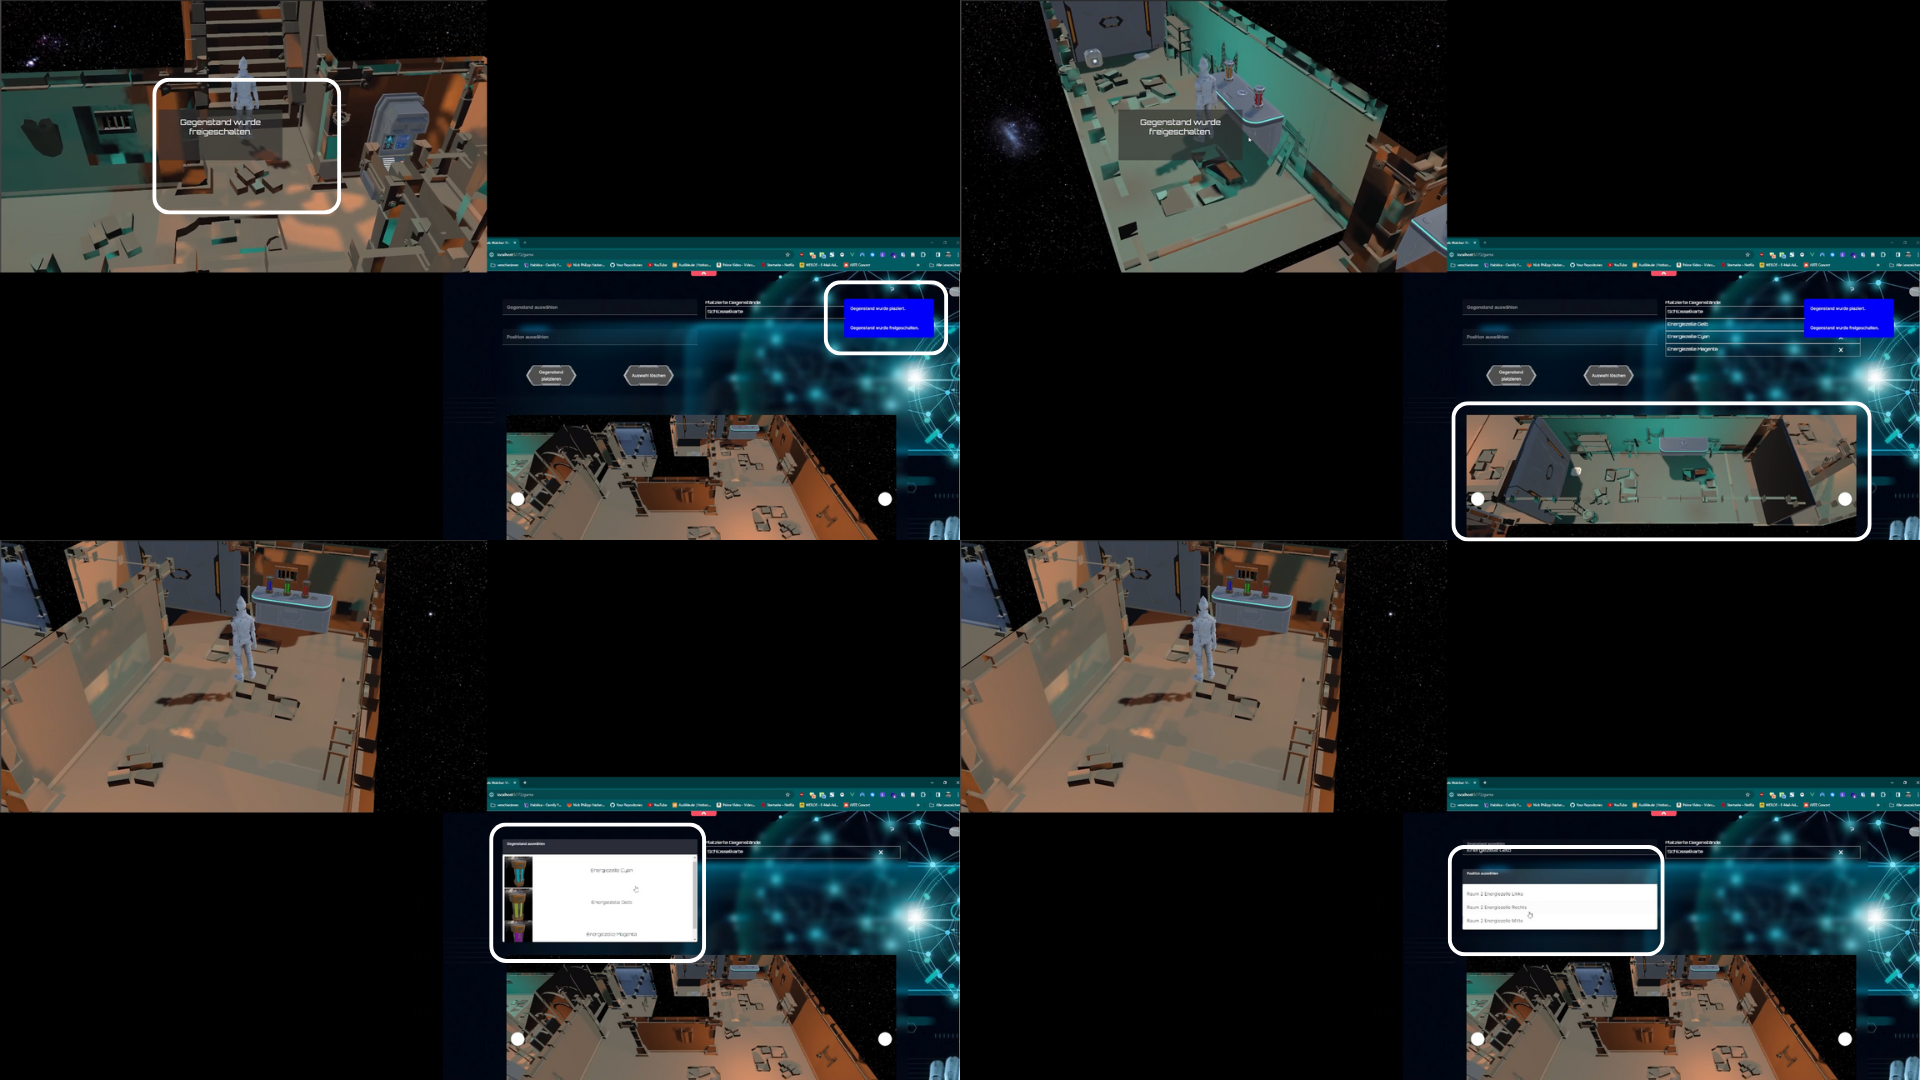
\includegraphics[width=1\linewidth]{content/pictures/UnlockMore.png}
\caption{Freischalten neuer Gegenstände (Quelle: eigene Darstellung)}
\label{fig:old-unlock-system}
\end{figure}

Sobald das Lösen des Rätsel das Hindernis beseitigt und einen neuen Bereich zugänglich macht, geht der Bilder-Slider in der Anwendung des Watchers auf das aktuelle Bild. Der Slider zeigt dem Watcher alle verfügbaren Abschnitte der Spielwelt (vgl. erste Reihe, rechtes Bild, in weiß umrandet in Abbildung \ref{fig:old-unlock-system}). Durch die neuen Spielabschnitte werden nicht nur neue Gegenstände freigeschaltet, sondern auch zusätzliche vordefinierte Positionen, auf denen die Gegenstände platziert werden können. Diese werden dem Watcher in den Gegenstand- und Positions-Dropdown aufgelistet (vgl. Abbildung \ref{fig:old-unlock-system}, beide Bilder in der zweiten Reihe in weiß umrandet). 

\subsection{Aspekte zum Überarbeiten}
\paragraph{Backfaces}
In den zuvor betrachteten Abbildungen \ref{fig:old-logins} bis \ref{fig:old-unlock-system} fällt auf, dass die Wände der Spielwelt, in der sich der Player befindet (jeweils immer das linke Bildelement), \say{eigenartig} aussehen. Das liegt daran, dass die einzelnen Raum-Elemente dafür gedacht sind, dass durch die Kameraperspektive der Spieler im inneren des Raumes zu sein sollte. Man müsste für diesem Raumaufbau eine First-Person Kameraansicht wählen.

\begin{figure}[ht]
\centering
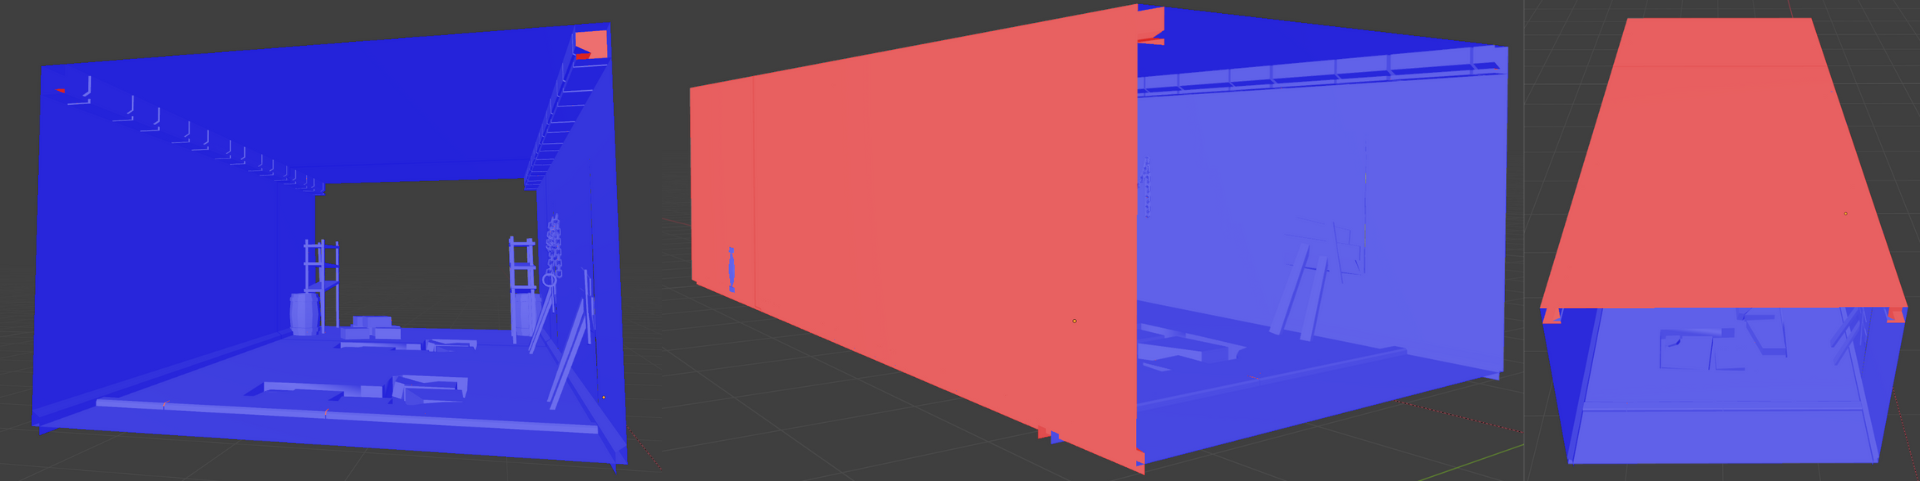
\includegraphics[width=1\linewidth]{content/pictures/Backfaces.png}
\caption{Fehlende Rückwand-Oberflächen in den Raummodellen (Quelle: eigene Darstellung), (Modell von \cite{alasl_autolevel_nodate})}
\label{fig:missing-backfaces}
\end{figure}

Abbildung \ref{fig:missing-backfaces} zeigt fehlende Rückseiten-Oberflächen an. Die blauen Oberflächen sind die Oberflächen, die durch ihre Ausrichtung der Normalvektoren von der Game-Engine gerendert werden können. Die roten Oberflächen sind die, die von der Game-Engine nicht berücksichtigt werden. Hierbei kann es zwei unterschiedliche Ansätze geben, fehlende Rückseiten hinzuzufügen. Innerhalb der Material-Konfiguration der einzelnen Materialien kann bi-direktionales Rendering aktiviert werden oder das Modell muss pro Richtung auf die auf das Modell geschaut wird jeweils eine Oberfläche haben, die auch in diese Richtung zeigt.

Außerdem müsste für den Anwendungszweck eines Spiel mit einer Top-Down Ansicht auch eine Decke der Räume entfernt werden, da diese für den Spieler nicht sichtbar sein sollte und sonst stören würde.

% backfaces

\paragraph{Steuerung des Avatars}
Im vorangegangenem Prototyp wurde wenig Aufmerksamkeit auf die Gestaltung der Spielsteuerung über Touch-Inputs gelegt. Die Standard-Steuerung innerhalb des verwendeten Unity-Assets von \cite{alasl_autolevel_nodate} enthielt zum Start des Projekts nur die Steuerung über Maus und Tastatur. Über die Tastatur konnte sich über die Spielwelt hinweg bewegt werden, ähnlich wie es aus \ac{RTS}-Spielen bekannt ist. Über die linke Maustaste konnte in die Spielwelt geklickt werden, wodurch sich der Spieler-Avatar an diese Stelle selbständig bewegte. Eine Steuerung über Touch-Eingaben an einem Touch-Monitor oder Fernseher musste erst eingebaut werden. Das Asset von \cite{alasl_autolevel_nodate} verwendet das Kamera-System der Cinemachine (vgl. \cite{noauthor_about_nodate}) wodurch einige vorgefertigte Steuerungen der Kamera durch die Maus bereits implementiert sind. 

Es fehlte also die Touchsteuerung. Diese wurde allerdings nicht nach den Funktionalitäten eines Touchscreens konzipiert und umgesetzt, wie es bspw. in der Arbeit von \cite[S. 64ff]{reinhard_augmented_2022} aufgezeigt wurde, sondern über eigene Ideen, die nicht den Komfort der Maussteuerung wiedergeben konnte. Durch existierende und nicht sichtbare Oberflächen in der Spielwelt, wurde ebenfalls die Erfolgschance den Avatar durch einen Touch-Klick in die Spielwelt zu bewegen vermindert, wodurch ebenfalls Spielkomfort verloren ging.

% steuerung beim Player

\paragraph{Interaktion mit der Spielwelt}
Sowohl die Anwendung des Players als auch die des Watchers besitzen wenig, bis keine Interaktionen mit der Spielwelt. Bei der Anwendung des Players besteht lediglich das Laufen innerhalb der Spielwelt als Interaktion. Der Watcher hingegen besaß keine Funktionalität im Bezug auf die Spielwelt. Lediglich die Menüs, über die die Daten der Session bearbeitet werden konnten. Für einen zukünftigen Prototyp müssen mehr Kernfunktionen in die Anwendungen eingebaut und Interaktionen mit der Spielwelt geschaffen werden.

% interaktion mit der spielwelt beim watcher
% feedback von den probandentests aufzählen

\paragraph{Sonstiges Feedback aus den Probandentests}
\begin{figure}[ht]
\centering
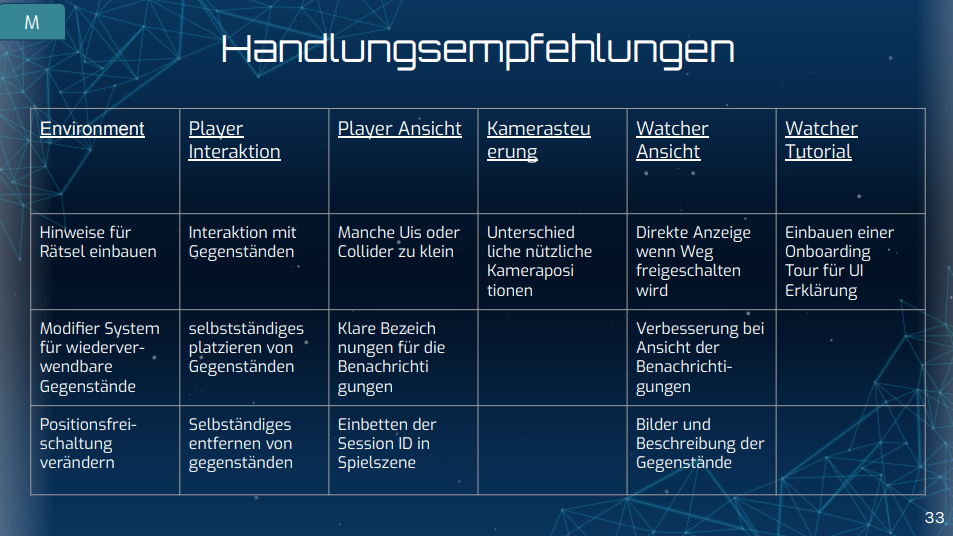
\includegraphics[width=1\linewidth]{content/pictures/Handlungsempfehlungen.PNG}
\caption{Handlungsempfehlungen des alten Prototyps (Quelle: eigene Darstellung aus der Abschlusspräsentation), (ganze Präsentation in Anhang \ref{}, S. 33)}
\label{fig:recommended-action}
\end{figure}

Abbildung \ref{fig:recommended-action} zeigt die Handlungsempfehlungen für den alten Prototyp aus der vorangegangenen Arbeit. Die Abschnitte der \say{Player Interaktion}, \say{Player Ansicht}, \say{Kamerasteuerung} und \say{Watcher Ansicht} wurden bereits angesprochen. Die Abschnitte \say{Environment} und \say{Watcher Tutorial} fehlen noch, wobei \say{Watcher Tutorial} in der Weiterentwicklung des Prototyps in der Implementierung keine Beachtung geschenkt wurde, da der Umfang ein eingebautes Tutorial für \ac{UI}-Elemente zu konzipieren und umzusetzen zu aufwändig wäre. Es müsste außerdem auch für die Anwendung des Player gälten.

Daher wird nun noch der Fokus auf das Environment gelegt. Die Handlungsempfehlungen beziehen sich in der Darstellung auf das bestehende System des Prototyps. Abstrahiert betrachtet ermöglicht eine grundlegende Weiterentwicklung der Anwendungen und des Environment neue Möglichkeiten wie Rätsel innerhalb der Spielwelt konzipiert und umgesetzt werden können. Dadurch kann es frei wählbare Positionen auf der Spielkarte geben, die nicht mehr vordefiniert sein müssen, oder dass bestehende Gegenstände auf irgend eine weise verändert werden müssen. Diese Aspekte könnten in einer neu Entwicklung des Environments anders aufgebaut werden.

\section{Verwendete Technologien}
In der folgenden Aufzählung werden alle externen Assets und Packages vorgestellt, welche in der Entwicklung des Prototyps verwendet wurden. Manche der Assets werden im Registry des Projekts nicht aufgezählt, da diese in einem Test-Projekt importiert und für den Gebrauch dieses Projekt in jeweilige Submodule editiert importiert wurden. 

\subsection{Unity Editor Version 2022.3.45f1}
Der Prototyp wurde mit der 2022.3.45f1 \ac{LTS}-Version umgesetzt, da diese zum Start der Masterarbeit die aktuelle 2022 \ac{LTS}-Version war. Zwischenzeitlich wurde auch die 2023.2.20f1 (vgl. \cite{noauthor_unity_nodate}) ausprobiert. Da diese allerdings weder eine \ac{LTS}-Version noch zusätzlich im Package der Cinemachine ein Major-Update enthalten war und die Cinemachine einige Probleme mit sich führte, wurde eine stabile 20222-Version gewählt.

\subsection{Blender 4.3.2}
Blender dient als Bearbeitungstool für die 3D-Modelle aus den hinzugenommenen Unity Assets. Die aktuelle Version zu Projektstart war die 4.3.2 Version- welche über den gesamten Bearbeitungszeitraum verwendet wurde. Außerdem bietet Unity einen Blender Direktimport an, wodurch keine \ac{FBX} oder \ac{OBJ} Dateien aus den Blenderdateien exportiert und in Unity importiert werden mussten.

\subsection{NuGetForUnity 4.1.1}
NuGetForUnity ist ein für Unity entwickelter NuGet-Client (vgl. \cite{noauthor_nuget_nodate}) über den zusätzliche funktionale Pakete für Unity installiert werden kann (vgl. \cite{mccarthy_glitchenzonugetforunity_2025}). Er war nötig, um ein nicht über Unity erworbenes Package in Unity nutzen zu können. Die aktuelle Version zum Bearbeitungsstart war die 4.1.1 Version, welche bis zum Ende genutzt wurde.

\subsection{Newtonsoft.Json 13.03}
Das erste Package, welches über NuGetForUnity installiert wurde ist Newtonsoft.Json, durch welches über den WebSocket übertragene JSON-Daten leicht deserialisiert und serialisiert werden können (vgl. \cite{newtonsoft_jsonnet_nodate}). Die aktuelle Version im NuGet-Paketverwaltungstool war die 13.03.

\subsection{WebSocketSharp-netstandard 1.0.1}
Derzeit gibt es einige Netzwerk-Integrationen für Unity, bspw. Mirror (vgl. \cite{noauthor_mirror_nodate}) oder Netcode for GameObjects (vgl. \cite{noauthor_about_2025}). Durch beiden Packages wäre jedoch die Netzwerk-Topologie starrer und die Entwicklung nach eigener Vorstellung wäre ebenfalls eingeschränkter. Daher wurde über NuGetForUnity das WebSocketSharp-netstandard Paket installiert, welches eine direkte Kommunikation mit einem WebSocket-Server ermöglicht (vgl. \cite{pingman_tools_pingmantoolswebsocket-sharp_2025}), da bislang existierende Integration mit Unity nicht mehr unterstützt werden. Die derzeit installierte und zum Projektstart installierbare Version ist die 1.0.1.

\subsection{AI Navigation 1.1.5}
Da sich der Avatar des Players innerhalb der Spielwelt per Touch-Click auf den Bildschirm an die angeklickte stelle bewegen soll, muss ein \ac{AI}-Agent eingebaut werden, der das Avatar Spielobjekt an die gewünschte Stelle bewegt. In Unity kann dafür das NavMesh System verwendet werden, welches ein Pathfinding-System implementiert, wodurch ein automatisiertes Bewegen eines Agents durch eine Zielposition integriert werden kann. Das Paket in Unity heißt dafür \ac{AI}-Navigation. Die aktuelle Version zum Start des Projekts ist die 1.1.5.

\subsection{Cinemachine 2.10.1}
Die Cinemachine wurde in der Entwicklung des Prototyps bei beiden Anwendungen als unterstützendes Element für die Kamerasteuerung verwendet. Durch die Cinemachine können virtuelle Kameras genutzt werden, durch welche verschiedene Ansichten in der Spielwelt erstellt werden können. Außerdem unterstützt sie bei der Kameraführung um ein verfolgtes Objekt, wie dem Avatar des Players. Zudem es ist durch sie möglich, auf einfache weise eine Zoom-Funktion einzubauen. Die aktuelle Version für die 2022-Unity Version ist die 2.10.1, welche über den Verlauf der Arbeit verwendet wurde.

\subsection{Universal RP 14.0.11}
Für die Entwicklung einer Anwendung für Mobile Endgeräte oder die für Windows-Geräte kann die \ac{URP} verwendet werden. Außerdem ist die \ac{URP} mit ARFoundation kompatibel, wodurch die Wahl auf die \ac{URP} und nicht die Built-In Render Pipeline fiel. Die zum Start und über den Verlauf der Arbeit genutzte Version ist die 14.0.11.

\subsection{Unity UI 1.0.0 und TextMeshPro 3.0.9}
Für die Entwicklung der \ac{UI}-Elemente der Anwendungen wurden die Pakete Unity \ac{UI} und TextMeshPro in ihren zum Start des Projekt aktuellen Versionen verwendet. Unity \ac{UI} ist dabei das Standard-Paket für die Entwicklung von User-Interfaces. TextMeshPro erweitert die Standard \ac{UI}-Elemente von Unity \ac{UI} um weitere Komponenten, welche für die Entwicklung des \ac{UI}s verwendet wurden.

\subsection{Input System 1.7.0}
Seit der 2022er-Unity Version wird empfohlen das neue Input System von Unity zu verwenden. Das alte Input System ist standardisiert in jedem Unity Projekt enthalten und wird durch das neue durch das Paket Input System überschrieben. Es ermöglicht über ein eigenes Menü verschiedene Input-Möglichkeiten zu konfigurieren und innerhalb der Scripte zu verwenden.

\subsection{FBX Exporter 4.2.1}
Manche Meshes der verwendeten Unity-Assets waren nicht im Binary-\ac{FBX}-Format importiert gewesen, wodurch sie über den \ac{FBX} Exporter zu einer Binary-\ac{FBX} Datei exportiert werden konnten. Außerdem kam es vor, dass manche Assets keine grundlegenden Meshes enthielten, wodurch die enthaltenen Prefabs zu \ac{FBX}-Dateien exportiert werden mussten. Die aktuelle Version des Exporters zum Start des Projekts war die 4.2.1.

\subsection{AR Foundation 5.1.6}
Für die Entwicklung von \ac{AR}-Anwendungen in Unity gibt es verschiedene Möglichkeiten. Die gängigsten Auswahlmöglichkeiten sind hierbei Vuforia (vgl. \cite{noauthor_home_nodate}) oder das Unity interne Paket AR Foundation (vgl. \cite{noauthor_ar_nodate}). Die AR Foundation ermöglicht im Vergleich zu Vuforia auf mehreren Arten das Tracking und Platzieren von virtuellen Gegenständen an, wodurch die Wahl auf die AR Foundation fiel. Außerdem ist die AR Foundation leichter in die Versionierung in Git einzubinden. Da gab es in vergangenen Projekten durch zu große Konfigurations-Dateien von Vuforia Problemen.

\subsection{Google ARCore XR Plugin 5.1.6}
In Abhängigkeit zum Paket AR Foundation wurde auch das Google ARCore Modul mit installiert, welches wichtig für mobiles \ac{AR} auf Android Smartphones ist. Es bietet eine Schnittstelle zwischen den Android eigenen Modulen auf dem Smartphone und der Unity Anwendung.

\subsection{Unity Assets}
Da durch den begrenzten Bearbeitungszeitraum keine Zeit blieb in großen Maßen eigene \ac{3D}-Objekte zu modellieren, wurde dafür auf bestehende und zum größten Teil kostenlose Assets zurückgegriffen, welche alle über den Unity Asset Store erworben werden konnten. Die enthaltenen Objekte wurden jedoch in einer großen Nacharbeitung an die eigenen Anforderungen angepasst und in die eigenen Submodule importiert.
\begin{itemize}  
    \item Astronaut - Free Model By Quaternius von \cite{quaternius_astronaut_nodate}
    \item Chair Pack - 3D Low Poly Office Furniture 1.0 \cite{fast_mesh_chair_nodate}
    \item low poly WD | 3D Props 1.1 \cite{squid_low_nodate}
    \item Adventure Game Environment Pack | URP | 3D Sci-Fi 1.0 \cite{unity_technologies_adventure_nodate-1}
    \item Adventure - Sample Game | Tutorials 3.0 \cite{unity_technologies_adventure_nodate}
    \item Bedroom / Interior - Low Poly assets | 3D Interior 1.1.6 \cite{fries_and_seagull_bedroom_nodate}
    \item Big Furniture Pack | 3D Furniture 1.3 \cite{vertex_studio_big_nodate}
    \item Chair pack - 3D Low Poly Office Furniture - Created with FastMesh Asset | 3D Furniture 1.0 \cite{fast_mesh_chair_nodate}
    \item Fantasy Cemetery \& Necropolis Pack Lite: 3D Assets for RPG and Adventure Games | 3D Fantasy 1.2 \cite{emaceart_fantasy_nodate}
    \item Free Wood Door Pack | 3D Interior 1.0 \cite{biostart_free_nodate}
    \item Kitchen Appliance - Low Poly | 3D Electronics 1.02 \cite{alstra_infinite_kitchen_nodate}
    \item Lowpoly Dungeon Assets | 3D Dungeons 1.0 \cite{kunniki_lowpoly_nodate}
    \item Low Poly Dungeon Generator | 3D Dungeons 1.0 \cite{mysticforge_low_nodate}
    \item Low Poly Dungeons Lite | 3D Dungeons 1.11 \cite{justcreate_low_nodate-1}
    \item Low Poly Simple Medieval Props | 3D Props 1.0 \cite{justcreate_low_nodate}
    \item LowPoly Server Room Props | 3D Environments 1.0 \cite{ipoly3d_lowpoly_nodate}
    \item Melon's Low Poly Office | 3D Interior 1.1.1 \cite{mistyczny_arbuz_melons_nodate}
    \item Office Pack - Free | 3D Interior 1.02 \cite{nappin_office_nodate}
    \item Ultimate Low Poly Dungeon | 3D Dungeons 2.0 \cite{broken_vector_ultimate_nodate}
\end{itemize}

\subsection{Node Version 20.18.1}
Für den WebSocket-Server wurde eine Laufzeitumgebung benötigt, welche die zum Zeitpunkt des zugrunde liegenden Projekts die Node 20.18.1 war. Da das Teilprojekt des WebSocket-Servers aus dem vorangegangenen Projekts wiederverwendet werden konnte, wurde die Node Version beibehalten.

\subsection{Express.js Webserver 5.1.0}
Express.js ist eine Webserver Erweiterung von Node.js Servern, durch welche spezifische \ac{URL}-Endpunkte erstellt werden können, über welche bestimmte Funktionen gestartet werden. Außerdem ist er die Basis des WebSocket-Servers durch welchen dieser erst erreichbar wird.
% \cite{noauthor_express_nodate}

\subsection{WS 8.18.2}
WS ist das \ac{NPM}-Paket, über welches der WebSocket-Server implementiert werden kann. Das Paket ist innerhalb eines Express.js Server einfach zu verwenden und ermöglicht es Nachrichten zu empfangen und zu senden. Außerdem können empfangene Nachrichten in einem internen Mechanismus weitergereicht werden, wodurch für verschiedene Nachrichten Arten verschiedene Klassen gebaut werden konnten (vgl. \cite{websockets_websocketsws_2025}).

\subsection{Docker}
Docker ist eine Open-Source-Plattform über die Container erstellt, bereitgestellt ausgeführt, aktualisiert und verwaltet werden können. Container sind standardisierte, ausführbare Komponenten, die den Code von einzelnen Anwendungen mit den Betriebssystembibliotheken und Abhängigkeiten kombinieren (vgl. \cite{noauthor_was_2024}). Docker wurde aus dem Grund eines möglichen späteren Deployments des WebSocket-Server verwendet, da aus dem erstellen Express.js Server ein Docker-Image erstellt werden könnte und so die öffentliche Bereitstellung vereinfacht worden wäre. Außerdem können über die Docker Engine weitere Images importiert werden, welche lokal auf dem Gerät laufen und so eine Unabhängigkeit zum Internetzugang bestehen kann.
% \cite{noauthor_docker_2025}

\subsection{MongoDB - Docker Image}
MongoDB bietet über das eigene Atlas System einen Online-Zugriff auf definierten Datenbanken an. Allerdings sind diese nur über das Internet erreichbar und können in der Datenanfrage und dem Daten zuschicken Latenzzeiten beinhalten. Daher wurde ein Docker Image für eine MongoDB Umgebung verwendet. Dieses Image ist aus der Docker Community und für jeden frei zugänglich (vgl. \cite{noauthor_mongo_nodate}). Diese läuft auf dem Rechner, auf dem Docker läuft und ist innerhalb dieses Rechners frei erreichbar.

\subsection{node-mongodb-native NPM-Paket}
Um innerhalb des Express.js Servers eine Verbindungen zur MongoDB Datenbank aufbauen zu können, existiert eine Library, die Zugänge und weitere Funktionen im Bezug auf MongoDB bereitstellt. Das \ac{NPM}-Paket \say{node-mongodb-native} wurde für diesen Zweck verwendet (vgl. \cite{mongodb_mongodbnode-mongodb-native_2025}).


\subsection{User Interface Inspirationen}
Für die bisherig Implementierten \ac{UI}-Elemente wurden bestehende Bilder oder Icons nachgezeichnet und als Vorlage für eine Weiterentwicklung des \ac{UI}s eingebaut. Im folgenden werden die Quellen aufgezählt.

\begin{itemize}
    \item Vorlage für SciFi \ac{UI}s von \cite{pchvector_free_nodate}
    \item Vorlage für Low-Poly Feder von \cite{masud_download_nodate}
    % [TODO: Hier fehlen noch die Dumps von CHat, die nachgemalt wurden]
    \item Vorlage für die Rucksack Icon in Anhang \ref{}
    \item Vorlage für das Positions zurücksetzen Icon \cite{noauthor_chatgpt_nodate-3}
    \item Vorlage für das Hinweis Icon \cite{noauthor_chatgpt_nodate-2}
    \item Vorlage für Interaktions Icon \cite{noauthor_chatgpt_nodate-1}
    \item Vorlage für die Bücher Icons \cite{noauthor_chatgpt_nodate}
    \item Vorlage für die Handzeichnung in Anhang \ref{}
\end{itemize}

\section{Aufbau des Prototyps}
Der Prototyp ist wie der zugrunde liegende Prototyp in drei Einzelprojekte unterteilt. Die drei Einzelprojekte, die des Players, Watchers und des Servers, werden wie auch das vorangegangene Projekt in den Aufbau der \ac{MVC}-Architektur eingegliedert. Die Server-Anwendung aus dem vorangegangenem Projekt konnte weitergeführt und weiterentwickelt werden und funktionierte so nur in dieser bestimmten Architektur. Außerdem wurde diese gewählt, da im vorangegangenem Projekt jedes Gruppenmitglied einen eigenen Umsetzungsteil abgeben musste und diese Architektur das getrennte Entwickeln ermöglicht.
% Die Projekte des Players, Watchers und des Servers werden wie im alten Prototyp in die \ac{MVC}-Architektur eingegliedert.

\subsection{Player-Anwendung}
Die Player-Anwendung dient als die eine der beiden \say{Views} in dem entworfenem System. Sie umfasst grundlegend die Spielwelt, in der sich der Player-Avatar zur Laufzeit des Spiels bewegt. Die Spielwelt ist dabei so aufgebaut, dass es in einem der Submodule des Projekts Basismodelle für die Spielwelt gibt, die jeweils als Prefab Variant in diesem Projekt angepasst werden kann. Dadurch wird gewährleistet, dass der Kern der Spielwelt in der Anwendung des Players als auch des Watchers identisch bleibt und nur die gewünschten Unterschiede eingebaut werden können.

\paragraph{Steuerung der Anwendung}
Ein Kern der Player-Anwendung ist die Steuerung des Avatars. Im Ursprungsprojekt war geplant, dass der Spieler die Anwendung an einem Touchmonitor, entweder einem kleinen oder einem Smartboard, spielen kann.

\cite{reinhard_augmented_2022} stellt heraus, dass Multitouch-Anwendungen Pan (Drag-Bewegung nach Links-Recht-Oben-Unten), Zoom, Yaw (Finger-Rotierend) und Pitch (Neigungswinkelveränderung) Steuerungselemente enthalten können. 

Das bedeutet für die Anwendung, dass nun bestimmt werden muss, wie die Ansicht auf die Spielwelt und des Avatars ist, der innerhalb der Spielszene beegt wird. Unity bietet für Kamerafahrten, Kameraführungen und Kamerasteuerungen ein kostenloses Paket an. Die Cinemachine bietet verschiedene Kamera-Arten an, unter anderem das Kamera-System der \say{Free-Look-Camera}, durch welche der Nutzer in den bereitgestellten Komponenten ein \say{Follow} und \say{Look-At} Objekt hinterlegen muss um sich frei um dieses Objekt bewegen zu können. Für diese Anwendung wäre das ideal, da nun automatisiert die Kamera dem Avatar folgen kann. Allerdings wird die Cinemachine bei Anwendungen mit Maussteuerung verwendet, da die Input-Actions der Maus direkt mit den Komponenten verbunden ist. Daher müssen nun die von Reinhard aufgezeigten Steuerungen eingebaut werden, damit die Cinemachine Free-Look-Camera auch mit einem Touchmonitor zu spielen ist. 

Die Pan-Geste, bei der mit einem Finger über den Bildschirm auf zwei Achsen vor/zurück oder nach rechts/links bewegt wird, eignet sich für die Drehung der Kamera um den Avatar. Sie ersetzt damit die Bewegung der Maus, durch welche um das Look-At Objekt gedreht wird. Da die Free-Look Komponente in der Mausteuerung auch automatisiert näher an das Objekt gefahren werden kann, muss die Funktion ebenfalls eingebaut werden. Die Zoom-Bewegung, bei der zwei Finger auf dem Bildschirm entweder zueinander oder voneinander weg bewegt werden, übernimmt die Kamerafahrt näher zum Objekt.

Es fehlt nun nur noch die Bewegung des Avatars. Dafür reicht die grundlegenden Single-Touch Touch Aktion, durch welche auf die Spielwelt geklickt wird und sich der Avatar zu dieser Position bewegen soll. Um die Bewegung des Avatars zu ermöglichen, wurde das System der NavMesh Agents verwendet. Das System ermöglicht durch einen Path-Finding Algorithmus dass sich der Agent selbständig an ein gewünschtes Ziel bewegen kann. Zunächst muss ein Surface der Spielwelt erstellt werden, anschließend kann dem Agent eine Zielposition übermittelt werden und der bewegt sich selbständig an die gewünschte Position. Durch das Follow der Cinemachine-Komponente folgt das Kamerasystem dem Avatar selbständig.

\paragraph{Questsystem}\label{sec:quest-system}
Da die Rätsel und Hindernisse nicht einfach irgendwie in der Spielwelt eingebaut wurden, wurde für diesen Zweck ein kleines System entworfen, durch welches verschiedene Rätsel zusammengebaut werden können.

\begin{figure}[ht]
\centering
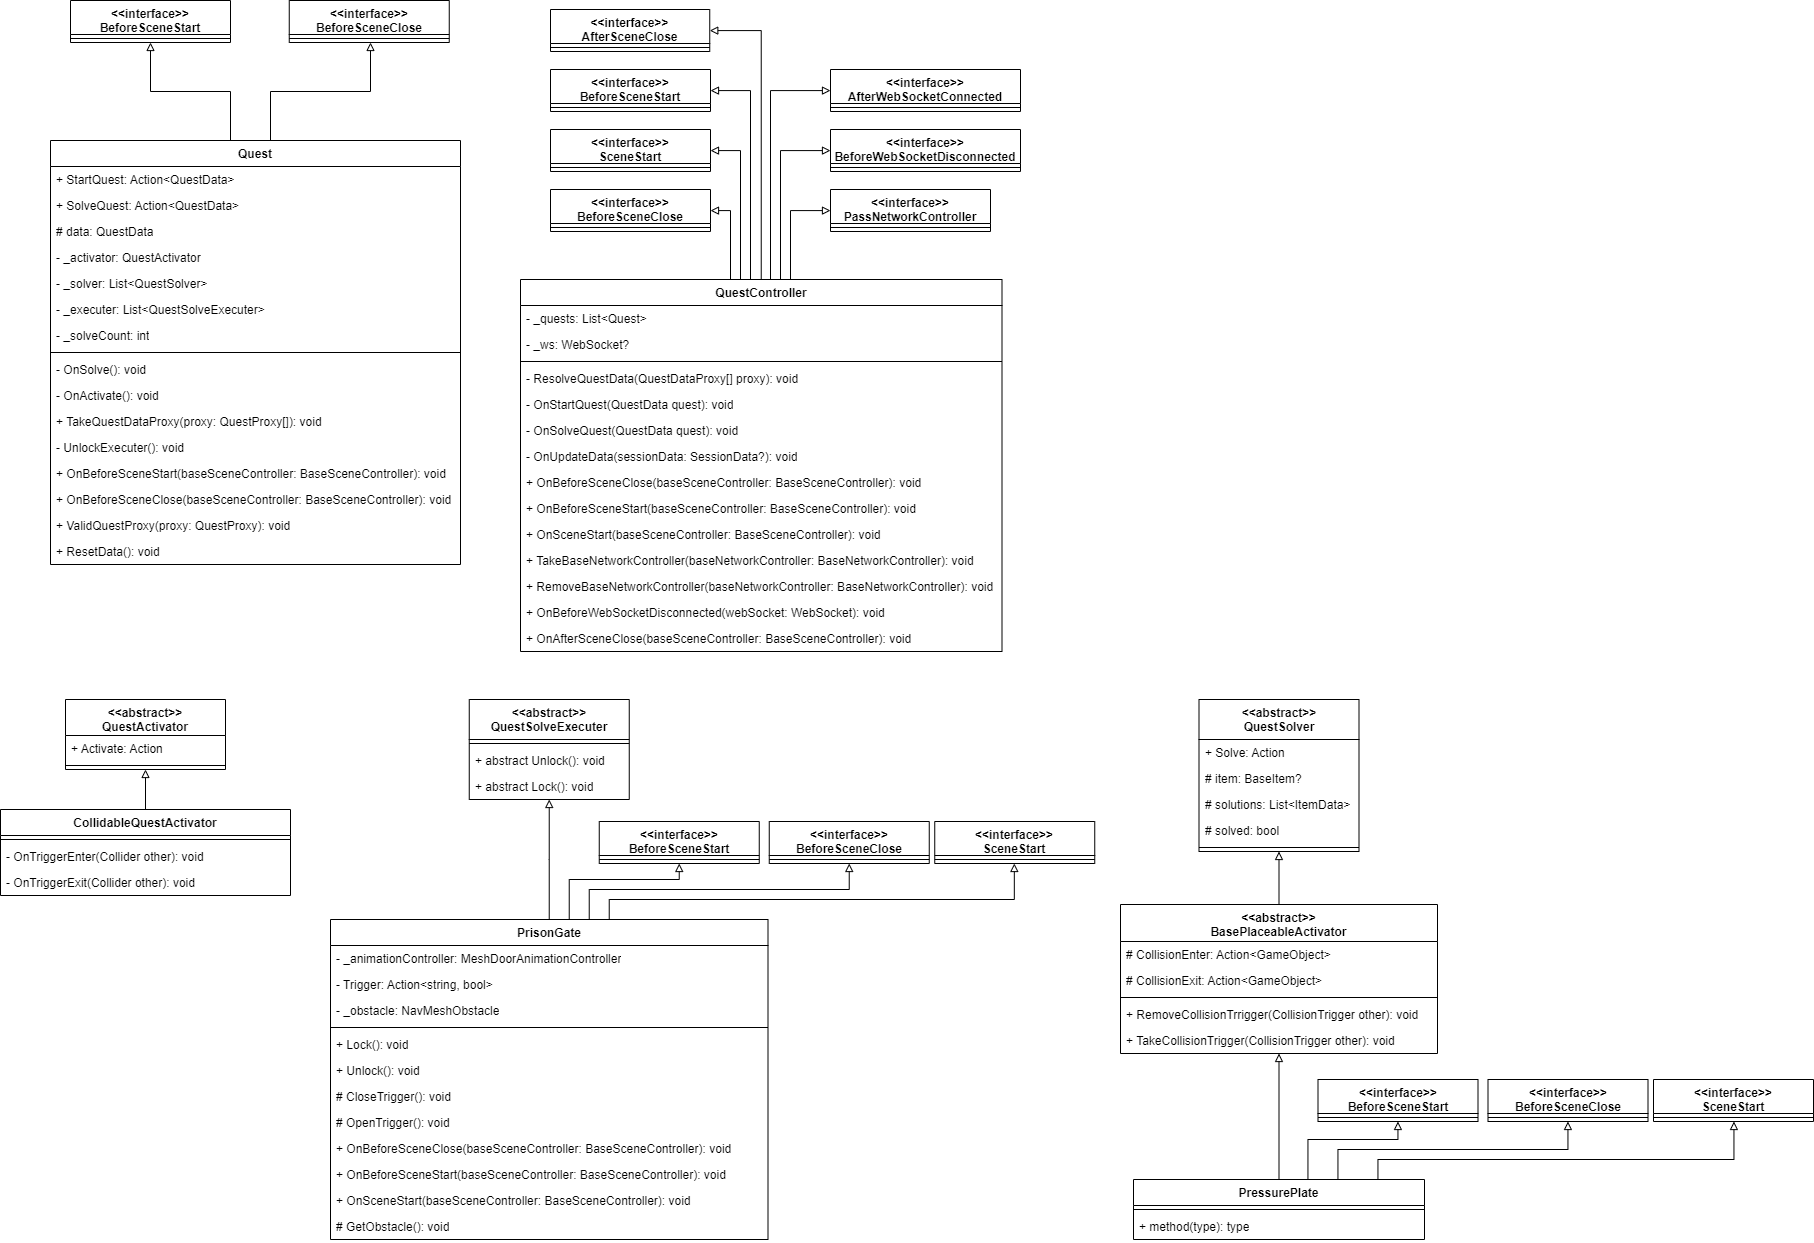
\includegraphics[width=1\linewidth]{content/pictures/QuestSystem.drawio.png}
\caption{UML-Diagramm zum Questsystem (Quelle: eigene Darstellung), (vollständig in Anhang \ref{})}
\label{fig:quest-system-uml}
\end{figure}

Abbildung \ref{fig:quest-system-uml} zeigt das entworfene \say{Questsystem}. Die einzelnen Herausforderungen wurden in Anlehnung an Quests aus \ac{RPG}-Spielen als solche benannt. Dieses System ist so modular aufgebaut, dass es sowohl in der Player- als auch in der Watcher-Anwendung eingebaut werden konnte. Die Inhalte dieses und des folgenden Kapitels gelten auch für die Watcher-Anwendung.

Der \say{QuestController} ist das überwachende Element innerhalb des Systems. Er besitzt zu allen \say{Quests}, die in der Spielszene erstellt wurden, eine Referenz. Er empfängt alle gelösten \say{Quests} vom Server und leitet diese an die jeweiligen \say{Quests} weiter. Außerdem ist er dafür verantwortlich, dass gelöste \say{Quests} an den Server übermittelt werden. Sobald eine neue \say{Quest} gestartet, also ein weiteres Rätsel freigeschaltet wurde, da ein weiterer Raum nun zugänglich gemacht wurde, leitet der \say{QuestController} diese ebenfalls an den Server weiter, damit diese zur Liste der bislang aktiven und zum Teil gelösten \say{Quests} hinzugefügt wird.

Die \say{Quest} für sich verteilt bestimmte Aufgaben an weitere Komponenten weiter. Sie besitzt ihre \say{Quest}-Daten, also ihren Namen, eine ID und ob sie gelöst wurde oder nicht, und überprüft sich selbst, ob sie gelöst wurde und würde dies an den \say{QuestController} weiterleiten. Damit die \say{Quest} weiß, ob sie gelöst wurde, besitzt sie Referenzen auf alles \say{QuestSolver}, die mit ihr in Verbindung stehen. Im Beispiel des Diagramms wäre es eine Druckplatte, die die Fähigkeiten eines Platzierungs-Aktivators hat, der aktiv wird, sobald innerhalb des eigenen Colliders ein richtiger Gegenstand platziert wurde. Sobald alle \say{QuestSolver} ausgelöst wurden, kann die Quest bestimmen, ob sie gelöst wurde. 

Bevor eine \say{Quest} gelöst werden kann, muss sie zunächst gestartet werden. Dies geschieht durch \say{QuestActivator}, zu welchen die \say{Quest} ebenfalls Referenzen besitzt. Werden alle Aktivatoren ausgelöst, so wird die \say{Quest} gestartet und kann gelöst werden. Im Beispiel der Abbildung existiert eine Komponente mit dem Namen \say{CollidableQuestActivator} die ausgelöst wird, sobald der Avatar des Players innerhalb des Colliders des Spielobjektes ist.

Nachdem die \say{Quest} gelöst wurde, führen alle mit der \say{Quest} verbundenen \say{QuestSolveExecuter} ihre jeweiligen Tätigkeiten aus. Jede \say{Quest} besitzt eine Referenz auf alle verbundenen \say{Executer}. Im Beispiel der Abbildung ist es eine Gefängnistür, welche beim Lösen einer \say{Quest} über den enthaltenen Animator aufgeht.

\paragraph{Pathsystem}\label{sec:path-system}
Wie das Questsystem wurde das Pathsystem ebenfalls möglichst modular gehalten, dass es auch in der Anwendung des Watchers eingebaut werden kann. Das Pathsystem ist deshalb wichtig, da zur Laufzeit des Spiels weitere Wege und Räume zugänglich gemacht werden und diese auf eine Weise mit der Logik der Rätsel verbunden sein müssen.

\begin{figure}[ht]
\centering
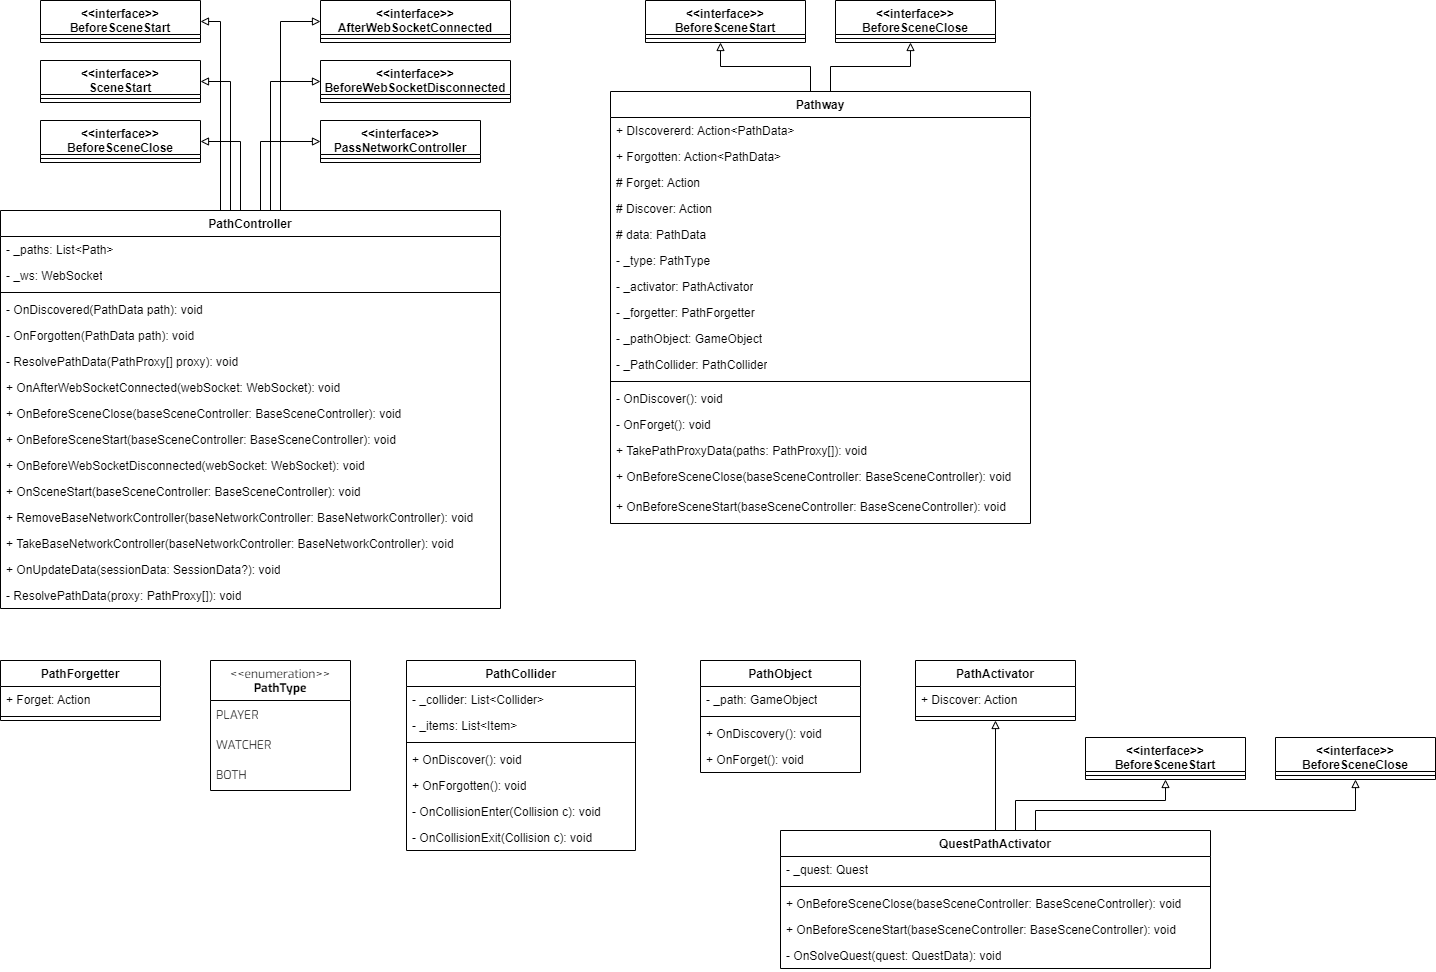
\includegraphics[width=1\linewidth]{content/pictures/PathSystem.drawio.png}
\caption{UML-Diagramm zum Pathsystem (Quelle: eigene Darstellung), (vollständig in Anhang \ref{})}
\label{fig:path-system-uml}
\end{figure}

Abbildung \ref{fig:path-system-uml} zeigt das entworfene modulares Pathsystem für die Player- und Watcher-Anwendung.

Wie auch im Questsystem, besitzt das Pathsystem mit der Klasse \say{PathController} ein überwachendes Element, das wie der \say{QuestController} dafür zuständig ist, Daten vom Server zu empfangen und an ihn zurückzusenden. Außerdem besitzt er Referenzen auf alle konfigurierten Wege der Spielwelt (\say{Pathways}). Erhält der \say{PathController} neue \say{Path}-Daten, werden diese an die jeweiligen \say{Pathway}-Komponenten weitergegeben.

Jeder \say{Pathway} besitzt Referenzen auf Aktivatoren (\say{PathActivator}) und Deaktivieren (\say{PathForgetter}), die je nach Anwendungsfall einen Weg entweder freischalten oder wieder deaktivieren. Zudem hat er zum eigentlichen Weg-Objekt, also dem Objekt, das in der Spielwelt diesen \say{Pathway} symbolisiert, und einer Collider-Klasse Referenzen. Diese werden jeweils bei Aktivierung und Deaktivierung des Weges relevant.

Da in dem konzipierten Tutorial kein Weg wieder deaktiviert wird, existiert dafür kein Beispiel. Die \say{QuestPathActivator}-Klasse ist im Beispiel des Diagramms dafür verantwortlich, nach Lösen einer \say{Quest} den mit dieser \say{Quest} verbundenen \say{Pathway} zu entdecken.

Wurde ein \say{Pathway} entdeckt, wird in der Komponente des \say{PathObjects} das entsprechende \ac{3D}-Objekt in der Spielszene aktiviert und die Collider für den Raum in der Komponente des \say{PathColliders} deaktiviert. Die Wichtigkeit der \say{PathCollider} wird im späteren Kapitel \ref{sec:difficulties-placement} erklärt. 

[TODO: ich müsste npch die Toolbar vom Player irgendwo zeigen]

\subsection{Watcher-Anwendung}
Die Watcher-Anwendung ist wie die Player-Anwendung eine der beiden \say{Views} der \ac{MVC}-Architektur. Auch sie umfasst die grundlegende Spielwelt aus der Sicht des Watchers und wie er mit dieser interagiert. In der Gestaltung der Spielwelt, wie sie der Watcher sieht gilt hier ebenfalls das gleiche wie beim Player. Sie enthält die Basisobjekte der Spielwelt, welcher innerhalb von Prefabs Variants editiert wurden.

Im Vergleich zum Player besitzt die Watcher-Anwendung jedoch zwei unterschiedliche Spielmodi. Der Watcher kann entweder mit der \ac{AR}-Integration einer Session beitreten oder über die \ac{3D}-Integration. Die \ac{3D}-Integration wurde grundlegend für die Entwicklung entworfen, da durch sie das Testen der bestehenden Entwicklungsstände einfach war. So musste die Anwendung nicht für das entsprechende Smartphone gebaut werden und konnte direkt im Editor getestet werden.

\paragraph{Steuerung der Anwendung}
Wie bereits in der Player-Anwendung ist auch hier ein großer Teil die Steuerung der Kamera innerhalb der Anwendung. Jedoch muss diese im Vergleich zur Player-Anwendung differenzierter betrachtet werden. 

In der \ac{AR}-Variante der Anwendung benötigt der Spieler keine umfassende Kamerasteuerung, da diese vom Smartphone \say{selbst} übernommen. \cite{reinhard_augmented_2022} zeigt dies in der Vorstellung der verschiedenen Touchsteuerungen aus (vgl. S.66ff). Der Spieler benötigt lediglich eine Single-Touch-Interaktion um mit der Anwendung interagieren zu können.

In der \ac{3D}-Variante muss, wie auch schon beim Player, auf die verschiedenen Steuerungsmöglichkeiten von \cite{reinhard_augmented_2022} zurückgegriffen werden. Zunächst ist jedoch zu entscheiden, welche Art von Kamerasystem die \ac{3D}-Anwendung haben soll. 

Einige Spiele für mobile Endgeräte besitzen keine freie Bewegung der Kamera. Manche besitzen ein Follow des Spieler-Avatars und der Rest besitzt keine freie Bewegung in der Spielwelt. Die häufigsten Umsetzungen für Steuerungselemente in Spielen für Touch-Endgeräte sind entweder die Steuerung über die verschiedenen Touch-Gesten, die \cite{reinhard_augmented_2022} in seiner Arbeit aufgelistet hat, oder Joystick-ähnliche \ac{HUD}-Elemente. 
So steuert der Spieler im Spiel \say{Botworld Adventure} (vgl. \cite{noauthor_botworld_nodate}) über Joystick-Elemente, oder in den Spielen \say{Die Sims Mobile} (vgl. \cite{arts_sims_2017}) und \say{Outlanders} (vgl. \cite{noauthor_outlanders_2025}) über verschiedene Touch-Gesten. 

Das Nutzen eines Joystick-Overlays würde den Sinn des Nutzens eines Touchmonitors nicht unterstützen, weshalb dieser Ansatz nicht weiter betrachtet wurde. Daher wurden die Kamerasysteme der anderen Steuerungsverwendungen betrachtet. In Sims Online und Outlanders wird ein ähnliches Kamera-System verwendet, wie es bereits aus Spielen wie der \say{Anno-Reihe} (vgl. \cite{noauthor_ubisoft_nodate}) bekannt ist. Sie nutzen ein sog. \say{Real-Time-Strategy}-System, bei dem die Kamera ein unsichtbares Objekt verfolgt, welches durch Nutzereingaben bewegt wird.

Der Ansatz der \ac{RTS}-Kameraführung wurde bei der Entwicklung der \ac{3D}-Anwendung verfolgt. Über die Single-Touch-Interaktion soll der Spieler Gegenstände platzieren können. Über die Yaw-Geste kann der Spieler die Ansicht auf die Spielszene drehen, um von einer anderen Blickrichtung neue Eindrücke sammeln zu können. Wie auch in der Player-Anwendung, kann der Spieler über die Zoom-Geste an die Spielwelt heranzoomen. Über die Pan-Bewegung kann der Spieler das \ac{RTS}-Kamerasystem durch die Spielwelt steuern. In der jetzigen Umsetzung gab es noch keinen Nutzen für die Pitch-Geste.

% [hier jetzt steuerungen von ein paar spielen nennen die es so gibt]
\paragraph{Aufbau des Nutzerflows}
Da die Hauptaufgabe des Watchers das Verwalten und Platzieren von Gegenständen ist, muss zunächst analysiert werden, wie ein für die Anforderungen an die Anwendungen passender Nutzerfluss konzipiert und umgesetzt werden kann.

Das Spiel \say{Outlanders} (vgl. \cite{noauthor_outlanders_2025}) passte in seinem Spielaufbau und seiner Führung durch die Menüs zu der Anforderung der Watcher Anwendung, bei der sich der Spieler zunächst frei durch die Spielwelt bewegen kann (entweder als \ac{AR}-Kamera oder über das RTS-Kamerasystem) und über ein Menü Gegenstände platzieren oder dem Player schicken kann.

In \say{Outlanders} muss der Spieler als Anführer der gemeinen Bevölkerung eine Stadt errichten. Dies kann er über ein Hauptmenü initiieren, welches sich in seiner Menüleiste befindet.

\begin{figure}[ht]
\centering
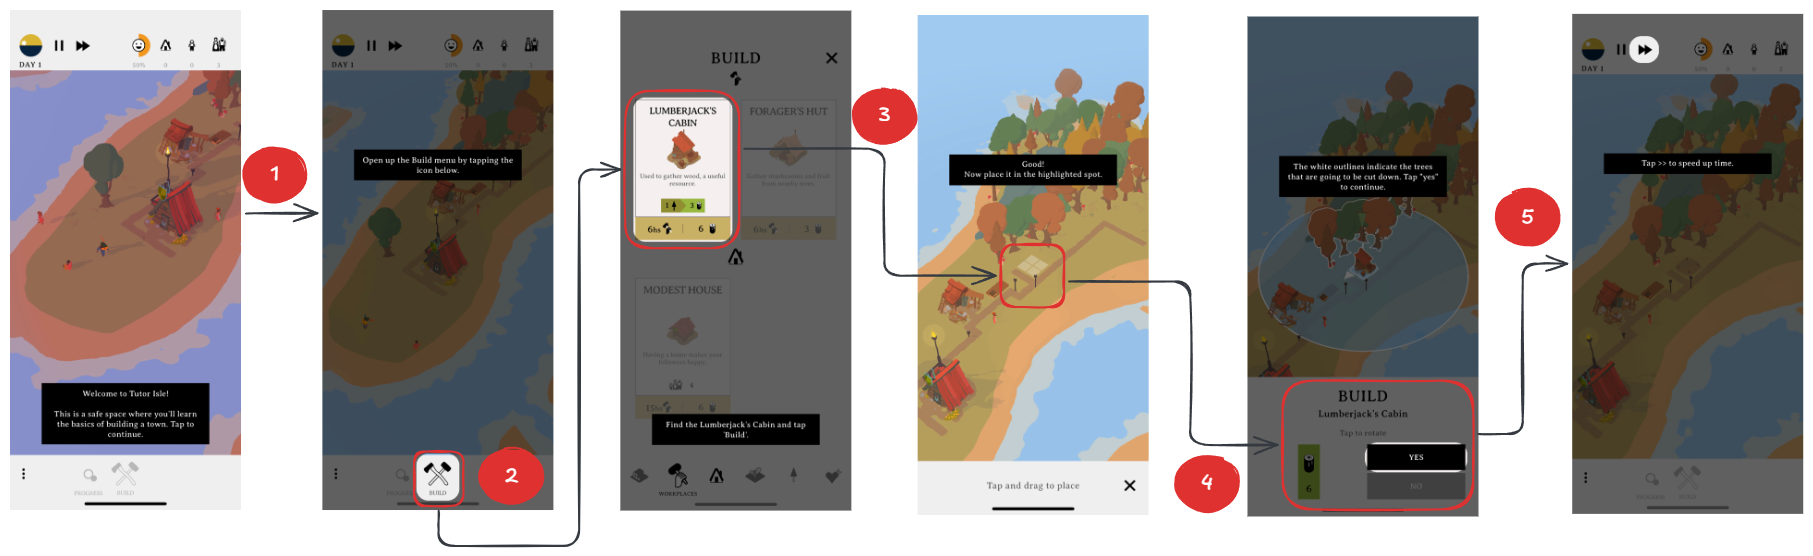
\includegraphics[width=1\linewidth]{content/pictures/Nutzerflow.png}
\caption{Nutzerfluss beim Gebäudebau in Outlanders (Screenshots von \cite{coates_game_nodate}), (Quelle: eigene Darstellung), (groß in Anhang \ref{})}
\label{fig:userflow-outlanders-build}
\end{figure}

Zunächst kann der Spieler sich frei durch die Spielwelt bewegen (1). Sobald der Spieler ein Gebäude für seine Bevölkerung bauen möchte, muss er in der Menüleiste am unteren Ende des Bildschirms auf den Reiter \say{Build} klicken (2). Darauffolgend öffnet sich ein Overlay-Menü, welches das Baumenü darstellt. In ihm kann der Spieler zwischen verschiedenen Kategorien von Gebäuden und anderen Bauelementen wechseln. Klickt er auf ein gewünschtes Gebäude, schließt sich das Menü und er muss nun in der Spielwelt auf die Stelle klicken, wohin das ausgewählte Gebäude platziert werden soll (3). Wurde eine Position gewählt, öffnet sich ein weiteres Menü, welches nur über die Hälfte des Bildschirmes geht, in welchem der Spieler bestätigen muss, dass das Gebäude an diese Stelle platziert werden soll (4). Nachdem er bestätigt hat, wurde das Gebäude platziert und das Bestätigungs-Menü geschlossen. Der Spieler kann nun wieder frei durch die Spielwelt navigieren (5).

Nicht nur der Nutzerfluss des Baumenüs wurde übernommen, sondern auch die Eindrücke des \ac{UI}s haben einen sehr starken Einfluss auf die ersten \ac{UI}s der Anwendung.

\begin{figure}[ht]
\centering
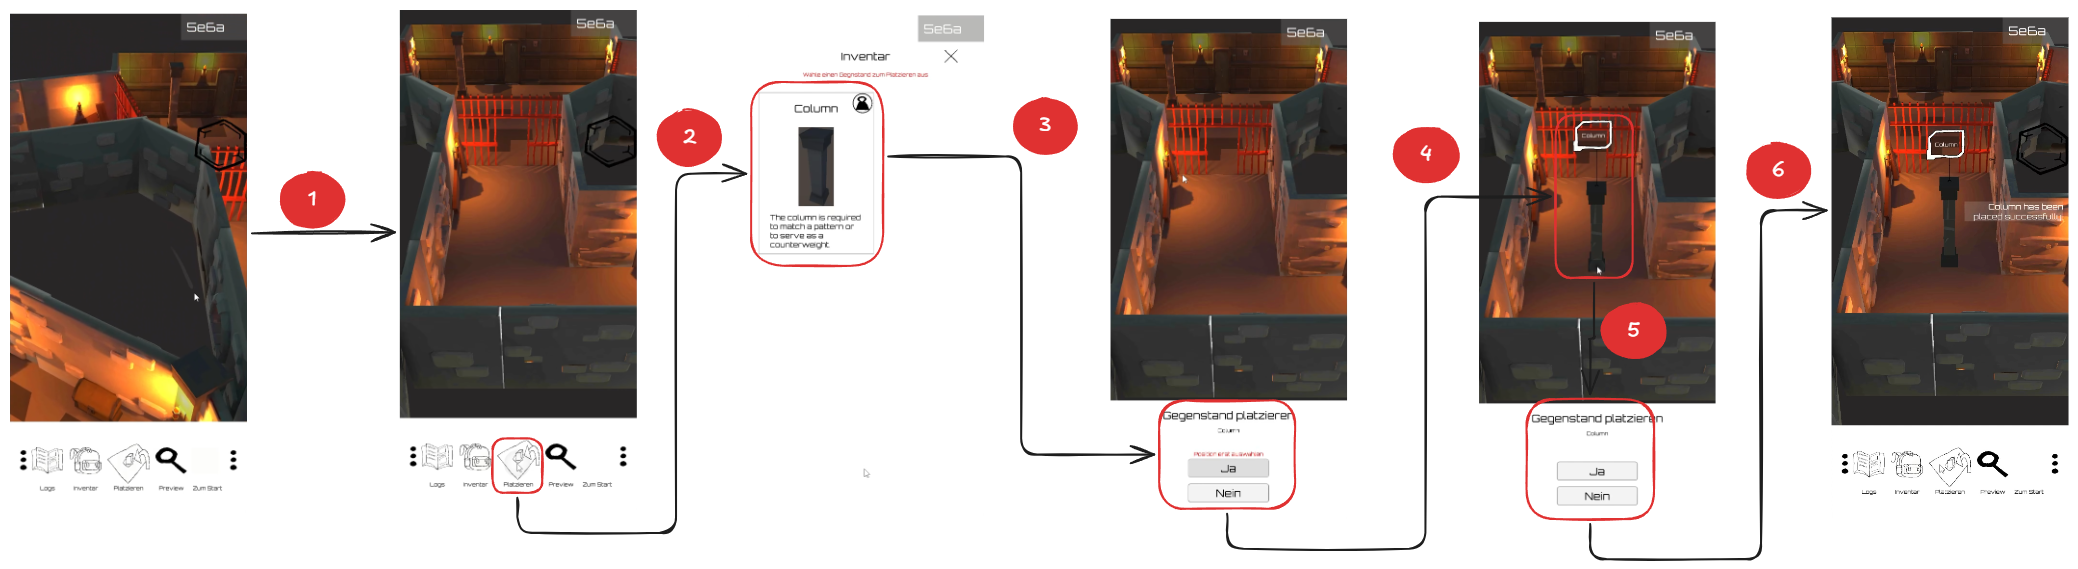
\includegraphics[width=1\linewidth]{content/pictures/PlacementFlow.png}
\caption{Nutzerfluss des Platzierens eines Gegenstandes (Quelle: eigene Darstellung), (groß in Anhang \ref{})}
\label{fig:userflow-placement-cm}
\end{figure}

Abbildung \ref{fig:userflow-placement-cm} zeigt den Nutzerfluss, den ein Spieler durchgeht, wenn er einen Gegenstand platzieren will. Er ähnelt sehr stark dem aus Outlanders. Zunächst kann sich der Watcher frei durch die Spielwelt bewegen (1). Nun muss er an einer bestimmten Stelle einen Gegenstand platzieren. Er klickt auf das Platzieren Menü und ein Overlay-Menü öffnet sich (2). Über das Menü kann er nun einen Gegenstand zum Platzieren auswählen (3). Sobald ein Gegenstand ausgewählt wurde, öffnet sich ein Menü, welches einen kleineren Teil des Bildschirms abdeckt und den Watcher auffordert eine Position zu wählen (3). Nachdem eine Position gewählt wurde, sieht der Watcher das zukünftig platzierte Objekt auf der gewählten Position (4). Über das noch aktive Menü kann der Nutzer nun die Platzierung des Gegenstandes bestätigen (5). Wurde die Wahl bestätigt, so steht nun an der gewählten Stelle der gewünschte Gegenstand (6). 

\begin{figure}[ht]
\centering
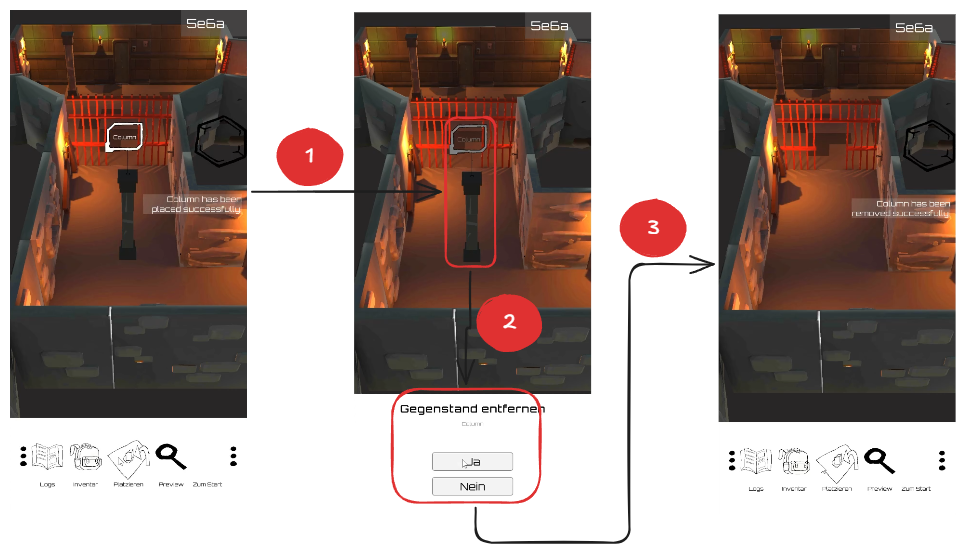
\includegraphics[width=1\linewidth]{content/pictures/RemovePlacementFlow.png}
\caption{Nutzerfluss des Entfernens eines Gegenstandes (Quelle: eigene Darstellung), (groß in Anhang \ref{})}
\label{fig:userflow-removement-cm}
\end{figure}

Abbildung \ref{fig:userflow-removement-cm} zeigt den Nutzerfluss, den ein Watcher durchläuft, sobald er einen platzierten Gegenstand wieder entfernen möchte. Zunächst kann sich auch hier der Watcher frei durch die Welt bewegen. Er muss nun aber einen Gegenstand entfernen, damit er ihn an einer anderen Stelle wieder platzieren kann. Er klickt nun auf den in der Spielwelt platzierten Gegenstand (1). Das Tooltip des ausgewählten Gegenstands verändert sich farblich, um dem Spieler zu zeigen, welcher Gegenstand ausgewählt wurde. Außerdem öffnet sich ein kleines Menü am unteren Ende des Bildschirmes, über welches der Watcher das Entfernen des Gegenstandes bestätigen kann (2). Nachdem das Entfernen bestätigt wurde, kann sich der Watcher wieder frei durch die Welt bewegen (3).

\begin{figure}[ht]
\centering
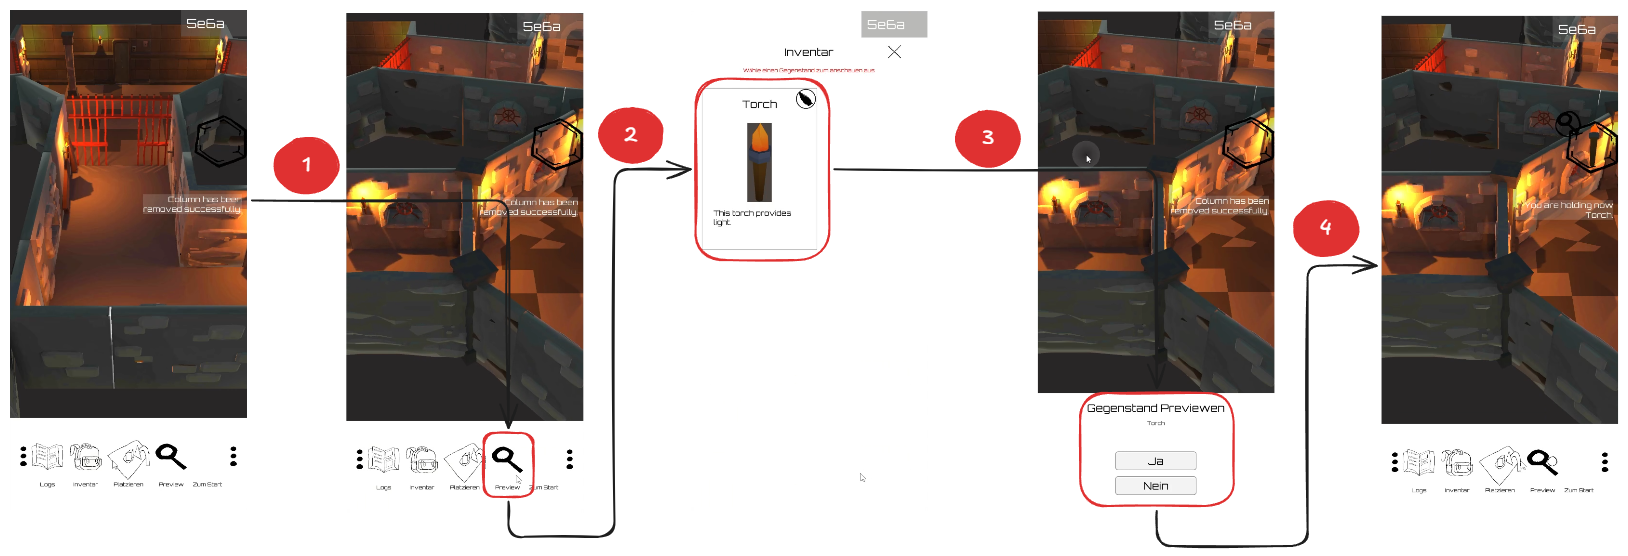
\includegraphics[width=1\linewidth]{content/pictures/PreviewFlow.png}
\caption{Nutzerfluss des Previewen eines Gegenstandes (Quelle: eigene Darstellung), (groß in Anhang \ref{})}
\label{fig:userflow-preview-cm}
\end{figure}

Neben dem Platzieren eines Gegenstandes ist auch das Schicken eines Gegenstandes an den Player eine wichtige Aufgabe des Watchers. Der vorangegangene Nutzerfluss aus der Vorlage von Outlanders und der bereits erfolgreichen Integration in den Nutzerfluss des Platzierens wurde dieser nun auch für das Previewen von Gegenständen eingesetzt (vgl. Abbildung \ref{fig:userflow-preview-cm}).

Nachdem sich der Watcher frei durch die Spielwelt bewegen konnte, muss er nun dem Player einen bestimmten Gegenstand schicken (1). Über das \say{Preview}-Menü, rechts neben dem \say{Platzieren}-Menü, kann der Watcher das Schicken initialisieren. Klickt er auf das Menü, öffnet sich auch hier eine Galerie, die über den ganzen Bildschirm geöffnet wurde. Hier kann der Spieler nun den gewünschten Gegenstand auswählen (2). Sobald ein Gegenstand ausgewählt wurde, öffnet sich ein Bestätigungsmenü, bei dem er die Auswahl bestätigen muss (3). Nachdem die Auswahl bestätigt wurde, kann sich der Watcher auch hier wieder frei durch die Welt bewegen und sieht dann der rechten, halb hohen Seite, den Gegenstand, den der Player nun trägt (4).

\begin{figure}[ht]
\centering
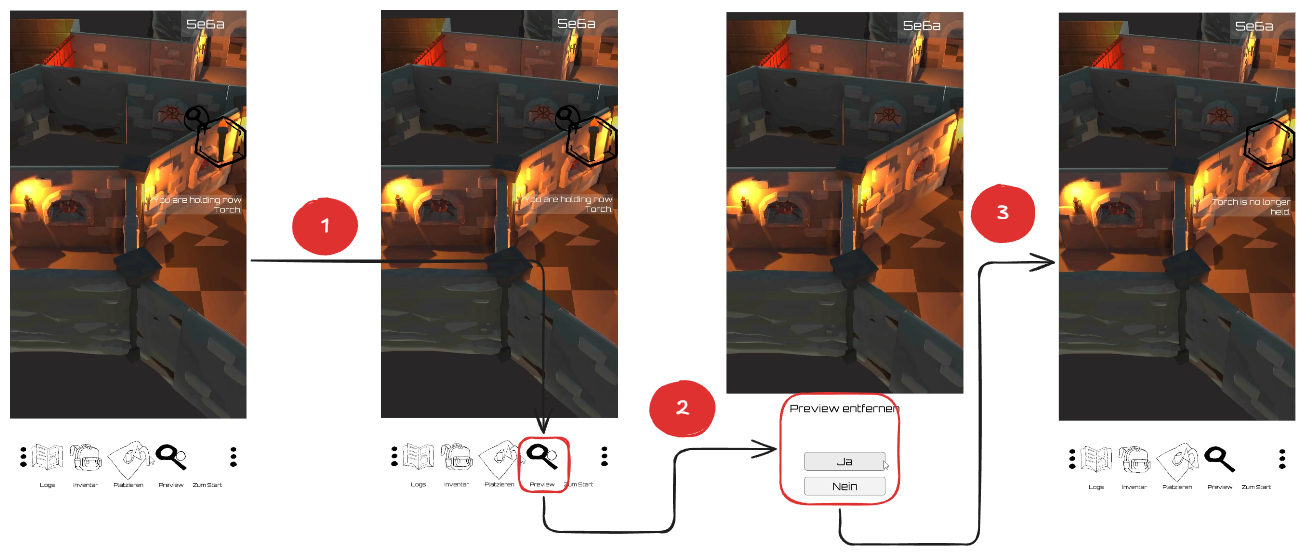
\includegraphics[width=1\linewidth]{content/pictures/RemovePreviewFlow.png}
\caption{Nutzerfluss des Entfernens der Preview eines Gegenstandes (Quelle: eigene Darstellung), (groß in Anhang \ref{})}
\label{fig:userflow-remove-preview-cm}
\end{figure}

Abbildung \ref{fig:userflow-remove-preview-cm} zeigt den Nutzerfluss des entsprechenden Entfernens der Preview eines Gegenstandes. Zunächst kann sich der Watcher noch frei durch die Welt bewegen. Sobald er einen Hinweis bekommt, dass er einen Gegenstand wieder entfernen soll, kann er wie beim Schicken eines Gegenstandes auf das \say{Preview}-Menü klicken (1). Nachdem er darauf geklickt hat, öffnet sich nicht wie beim ersten Mal ein Menü, sondern direkt das Überprüfungs-Menü, ob er den Gegenstand, den der Player gerade trägt, entfernen will (2). Bestätigt er das entfernen, so kann er sich wieder frei durch die Spielwelt bewegen. Außerdem wird der Gegenstand an der Rechten-Halbhohen Seite auch nicht mehr angezeigt (3). 

% spielwelten
% zwei versionen innerhalb des projekts 3D/AR
% bezug auf später bezüglich ar
% steuerungen in ar und 3d erwähnen mit bezug auf maps paper
% quest/ path system

\subsection{Server-Anwendung}
% netzwerk topologie vorstellen (relay-system)
% vorstellen der prototkolle und warum udp
Die Server-Anwendung ist, wie bereits in der Einleitung zu diesem Kapitel erwähnt wurde, das zentrale Element der \ac{MVC}-Architektur ist. 

Nun stellt sich die Frage, auf welche weise und durch welche Netzwerkprotokolle wird die Kommunikation zwischen den Anwendungen aufgebaut. Zunächst muss die Art des Servers bestimmt werden. Über den Aufbau der \ac{MVC}-Architektur geht hervor, dass die View getrennt vom Model und vom Controller steht, das beutetet, dass ein eigenständiges System für den Server geschaffen werden muss, mit dem die einzelnen Views kommunizieren können. Die in den Grundlagen der Netzwerkinfrastrukturen vorgestellten Ansätze können anhand der Architektur-Anforderung nun schematisch aussortiert werden. 

\paragraph{Bestimmung der Netzwerk-Topologie}

Eine klassische Client/ Server Netzwerkinfrastruktur kann ausgeschlossen werden, da weder der Server noch ein bestimmter Client als Server die Simulation der Spielwelt soll. Die einzelnen Views übernehmen das für sich und geben nur Veränderungen in den Kern-Datenelementen an den Server weiter. 

Ein \ac{P2P}-Modell ist in diesem Anwendungsfall auch nicht zielführend, da jede Anwendung mit den anderen Anwendungen verbunden sein müsste. Es würde ein zu großes Kommunikationsnetz mit aktualisierten Spielzuständen geben, welche ab einer bestimmten Spielgröße nicht mehr gewährleistet werden kann. 

Übrig bleiben daher nur noch das Modell der \say{distributed authorities} und das Relay-System. Eine Relay-Architektur unterstützt eine Multiplayer-Anwendung, bei der kein dedizierter Spielserver verwendet werden muss, der die Spiellogik simuliert. Er ist nur für die Kommunikation zwischen den verbundenen Anwendungen zuständig. Im Modell der distributed authorities ist jeder verbundene Client für die Simulation der Spielwelt selbst verantwortlich ist. Sie geben aktualisierte Spielzustände an einen Service weiter, der einen Überblick über den gesamten Spielzustand besitzt und gibt diesen an die anderen verbundenen Clients weiter. Die Kombination aus beiden Modellen wäre die ideale Architektur für den Spielserver von Connecting-Minds.

\paragraph{Bestimmung der Kommunikationsprotokolle}

\begin{figure}[ht]
\centering
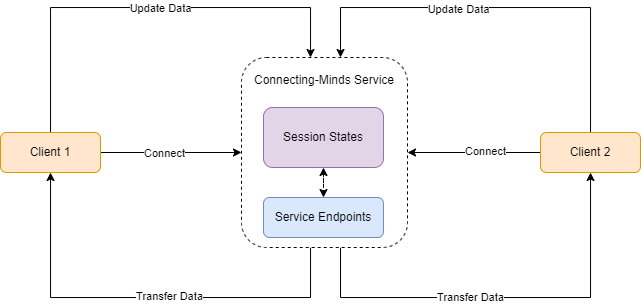
\includegraphics[width=1\linewidth]{content/pictures/CM-Archticture.png}
\caption{Connecting-Minds Infrastruktur (Quelle: eigene Darstellung)}
\label{fig:cm-topology}
\end{figure}

Nachdem eine Topologie bestimmt werden konnte (vgl. Abbildung \ref{fig:cm-topology}), muss nun bestimmt werden, auf welche weise die Anwendungen im Detail miteinander kommunizieren. 

% Durch das \ac{OSI}-Modell 
Das \ac{OSI}-Modell zeigt auf, welche verschiedenen Schichten in der Netzwerkkommunikation durchlaufen werden können (vgl. \cite{noauthor_osi-modell_nodate}). Jede Netzwerkkommunikation zwischen Anwendungen muss dabei durch den Transport-Layer der jeweiligen Endgeräte gehen. Innerhalb dieser Transportschicht existieren einige Protokolle, die den Transport der versendeten Datenpakete übernehmen. Die am häufigsten verwendeten Protokolle sind dabei das \ac{UDP} und das \ac{TCP} (vgl. \cite{noauthor_transport_nodate}). 

\begin{figure}[ht]
\centering
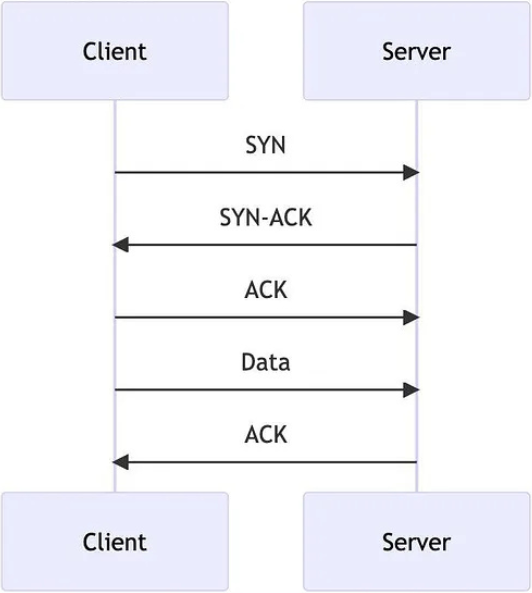
\includegraphics[width=0.5\linewidth]{content/pictures/TCP-Network.png}
\caption{Kommunikationsverbindung über TCP (Quelle: \cite{mygames_unity_2024})}
\label{fig:tcp}
\end{figure}

% Abbildung 
\ac{TCP} ist ein verbindungsorientiertes Protokoll, das zunächst eine Verbindung zu seinem Kommunikationspartner aufbaut, um Daten auszutauschen. Durch die Verbindung gewährleistet es einen zuverlässigen Datenaustausch, bei dem auch alle übertragenen Daten in der richtigen Reihenfolge beim Empfänger ankommen. Abbildung \ref{fig:tcp} zeigt diesen Verbindungsaufbau.
Zunächst erstellen der Client und Server einen Socket, um Daten über \ac{TCP} auszutauschen. Im Anschluss sendet der Client ein \ac{SYN}-Segment an den Server mit einem gewünschten Zielport. Anschließend akzeptiert der Server das \ac{SYN}-Segment, erstellt einen eigenen Socket und sendet an den Client ein \ac{SYN}-\ac{ACK}-Segment zurück. Der Client beantwortet dies mit einem \ac{ACK}-Segment. Nun besteht eine bidirektionale Verbindung  (vgl. \cite{mygames_unity_2024}).

% Einen \say{Distributed Authority} Ansatz kann es im Aufbau des Prototyps nicht gehebn
\ac{UDP} ist ein einfacheres Protokoll als \ac{TCP}, es garantiert weder die Zustellung noch die Reihenfolge der versendeten Pakete. Es baut zudem keine Verbindung zu seinem Kommunikationspartner auf, sondern sendet diese direkt an den Kommunikationsteilnehmer. Dadurch ist es wesentlich schneller als \ac{TCP} und wird häufig in Online-Spielen verwendet, die eine Echtzeitdatenübertragung erfordern (vgl. Abbildung \ref{fig:udp}). Da \ac{UDP} keine Zustellung garantiert, benötigt die Verwendung eine sorgfältige Handhabung (vgl. \cite{mygames_unity_2024}).

\begin{figure}[ht]
\centering
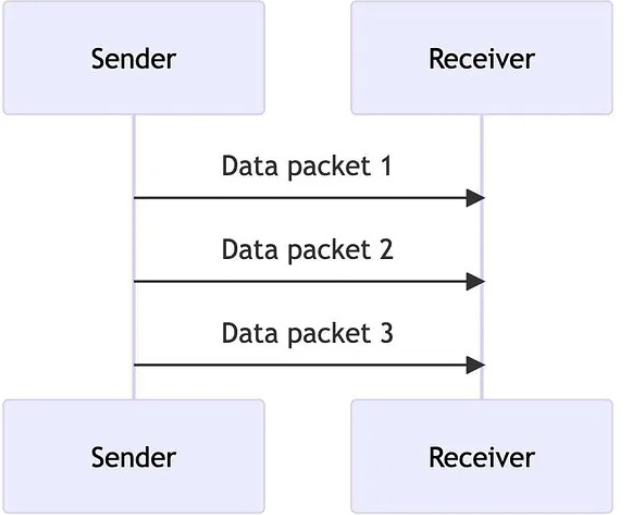
\includegraphics[width=0.5\linewidth]{content/pictures/UDP-Network.png}
\caption{Kommunikation über UDP (Quelle: \cite{mygames_unity_2024})}
\label{fig:udp}
\end{figure}

Auf Basis der Grundprotokolle \ac{TCP} und \ac{UDP} existieren auch Erweiterungen zu diesen. So ist das WebSocket Protokoll ein Application-Level Protokoll, das auf \ac{TCP} basiert. Es ermöglicht eine Erstellung einer Verbindung zwischen zwei Kommunikationsteilnehmern (etwa einem Browser und seinem Server). Im Vergleich zum \ac{HTTP}-Protokoll ermöglicht es eine bidirektionale Kommunikation zwischen den Teilnehmern. So kann der Server seinen Clients Nachrichten senden, ohne dass zuvor eine \ac{HTTP}-Nachricht versendet wurde (vgl. \cite{mygames_unity_2024}).

\begin{figure}[ht]
\centering
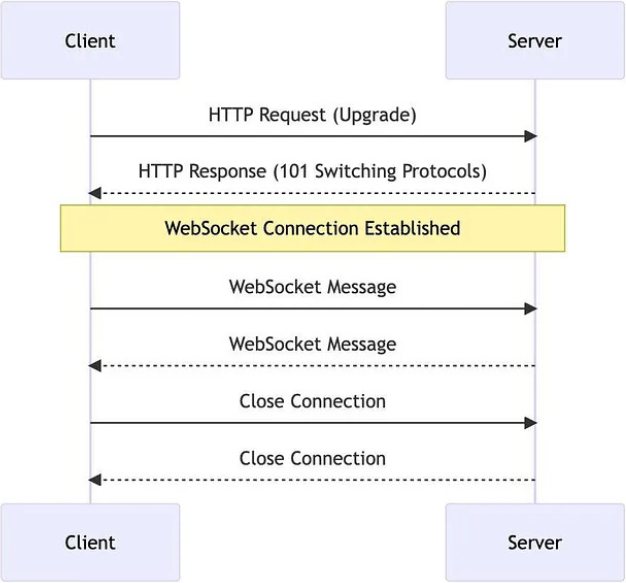
\includegraphics[width=0.5\linewidth]{content/pictures/WebSocket-Network.png}
\caption{Kommunikation über WebSocket (Quelle: \cite{mygames_unity_2024})}
\label{fig:ws}
\end{figure}

Für die entworfene Topologie ist die Kommunikation über das WebSocket-Protokoll das geeignetste. Es besteht eine persistente Verbindung der einzelnen verbundenen Anwendungen zum Server, welcher je nach Zustandsänderung an alle mit der Spielsitzung verbundenen Teilnehmer die Änderungen mitteilen kann. Dabei müssen sich die Teilnehmer nicht um eine Aktualisierung ihrer Zustände kümmern und erhalten zu jeder Zeit ein Update vom verbundenen Server (vgl. Abbildung \ref{fig:ws}).

\paragraph{Einbettung des Servers}

\begin{figure}[ht]
\centering
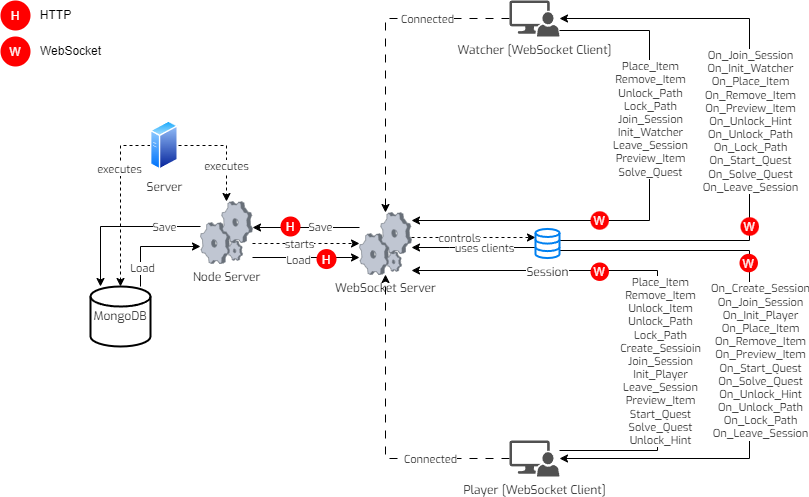
\includegraphics[width=1\linewidth]{content/pictures/Server-System.png}
\caption{Aufbau des Server (Quelle: eigene Darstellung)}
\label{fig:cm-server}
\end{figure}

Abbildung \ref{fig:cm-server} zeigt den Aufbau des Servers. Der physische Server führt dabei eine MongoDB Datenbank und einen Node-Server aus. Die MongoDB wird für die persistente Speicherung der einzelnen Sessions verwendet. Der Node-Server ist das Basis-Element der Server-Anwendung, da dieser den WebSocket Server startet, mit welchem sich die Spielteilnehmer verbinden werden. Der WebSocket Server ist zu dem dafür zuständig, dass durch die Aufforderung des Players neue Sessions erstellt werden. Wurde eine Session erstellt, wird der Player ihr automatisch beitreten. Ein Watcher kann nun ebenfalls der Session über den WebSocket Server beitreten. Die einzelnen mit dem Server verbundenen Clients kommunizieren nun über den Server mit der entsprechenden Session, welche über den Server Informationen zurückgibt. Die Clients kommunizieren dabei über das genannte WebSocket Protokoll.

Werden Sessions verlassen, werden diese vom WebSocket Server gespeichert. Dies geschieht durch \ac{HTTP}-Anfragen an den Basis Node-Server, welcher über seine Endpunkte die entsprechenden Daten abspeichert. Sie können durch das Beitreten einer bereits existierenden Session wieder geladen werden. Senden Player als auch Watcher eine Beitritts-Anfrage an den WebSocket-Server, so lädt dieser über den Node-Server und den entsprechenden Endpunkt diese Session und lässt die Anfrager, sofern eine Session gefunden wurde, beitreten.

% \paragraph{Vorstellung der Datenmodelle}

\section{Herausforderungen in der Umsetzung}\label{sec:difficulties}
Die Umsetzung einer Spielidee stellt oft im Verlauf des Entwicklungsprozesses Hürden bereit, welche auf verschiedenste Weisen gelöst werden müssen. Auch  diese Arbeit ist davon nicht verschont gewesen und stieß auf so manche Herausforderungen. 

\subsection{Erste Schritte im Leveldesign}
Zu Beginn der Schaffung der Spielwelt wurde überlegt, wie die Spielwelt auf einfache weise gebaut werden kann, damit sich hinterher nur noch überlegt werden muss, wie die enthaltenen Rätsel aussehen können. Um einzelne Spielräume generativ bauen zu können, wurde das Unity-Package von \cite{alasl_autolevel_nodate} näher betrachtet.

Das Asset umfasst einen Level-Builder, der aus den konfigurierten Modellen aus einem Repository generativ eine Spielwelt baut. Abbildung \ref{fig:level_builder} zeigt ihn in der Anwendung. Der Nutzer kann innerhalb des bestimmten Rasters einzelne Teile auswählen und dem Generator mitteilen, dass manche Stellen einen Hohlraum oder zusätzliche Elemente aus anderen Repositorys haben sollen.

\begin{figure}[ht]
\centering
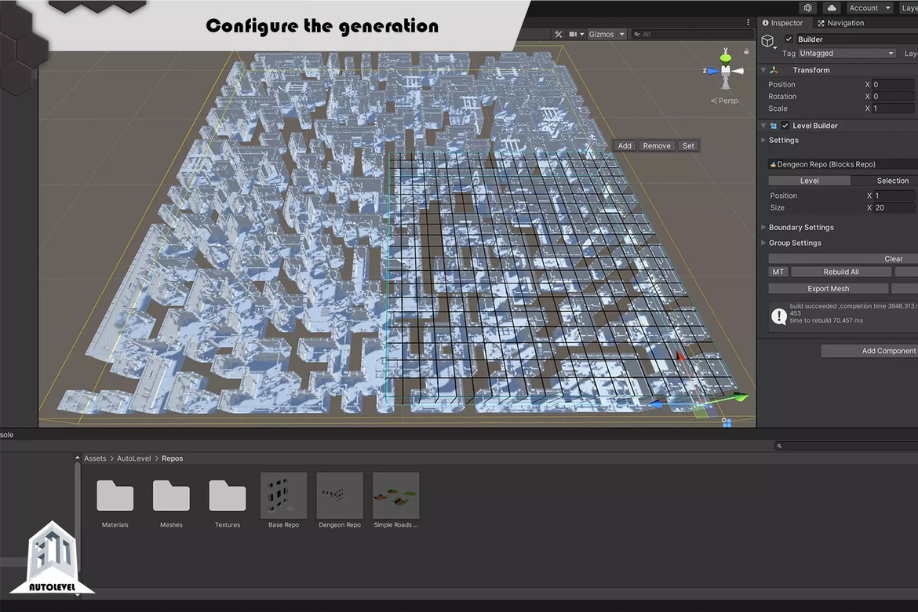
\includegraphics[width=1\linewidth]{content/pictures/FirstSteps00.png}
\caption{Level Builder Komponente (Quelle: \cite{alasl_autolevel_nodate})}
\label{fig:level_builder}
\end{figure}

Abbildung \ref{fig:level_builder_edit} zeigt dies anschaulich. Eine Teilfläche um das obere Ende des Level-Builder-Umfangs wurde über ein Menü des Builders ausgewählt und soll nun eine Anweisung für den Generator erhalten. In diesem Fall kann der Nutzer nun dem ausgewählten Bereich eine \say{Empty}Eigenschaft geben, sodass an dieser Stelle kein Raum generiert wird.

\begin{figure}[ht]
\centering
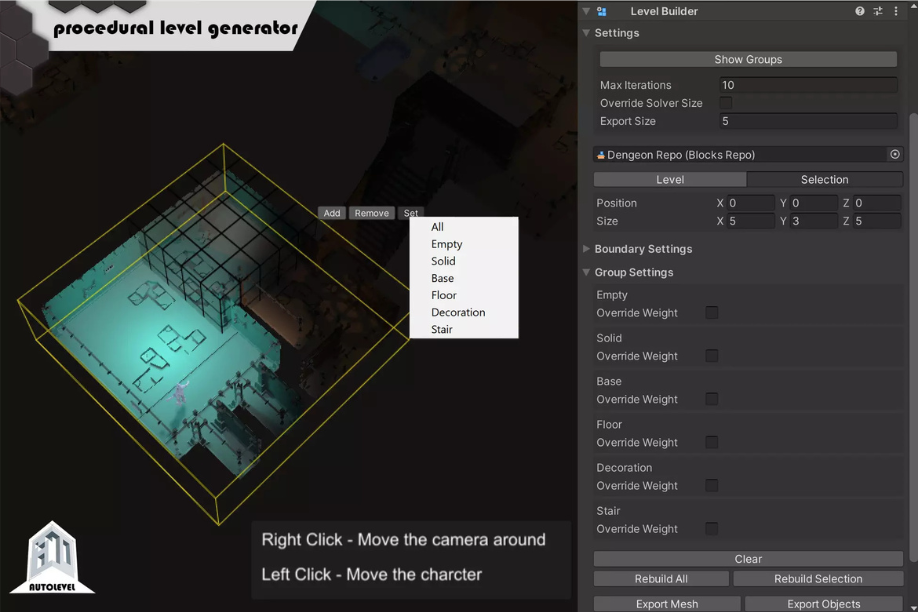
\includegraphics[width=1\linewidth]{content/pictures/FirstSteps01.png}
\caption{Level Builder Komponente (Quelle: \cite{alasl_autolevel_nodate})}
\label{fig:level_builder_edit}
\end{figure}

Um das Generieren der Spielwelt zu ermöglichen, muss zunächst ein Repository an Objekten erstellt werden, welche der Algorithmus verwendet. Ein Repository besteht aus einzelnen verschieden aussehenden 1x1x1 Meter großen modulare Einzelteile, die über das in Abbildung \ref{fig:repository-generator} gezeigte Menü zusammengesteckt werden können. So können aus den sechs Einzelteilen in der Abbildung viele verschiedene 2x3 große Teile ergeben, welche der Level Builder generieren kann.

\begin{figure}[ht]
\centering
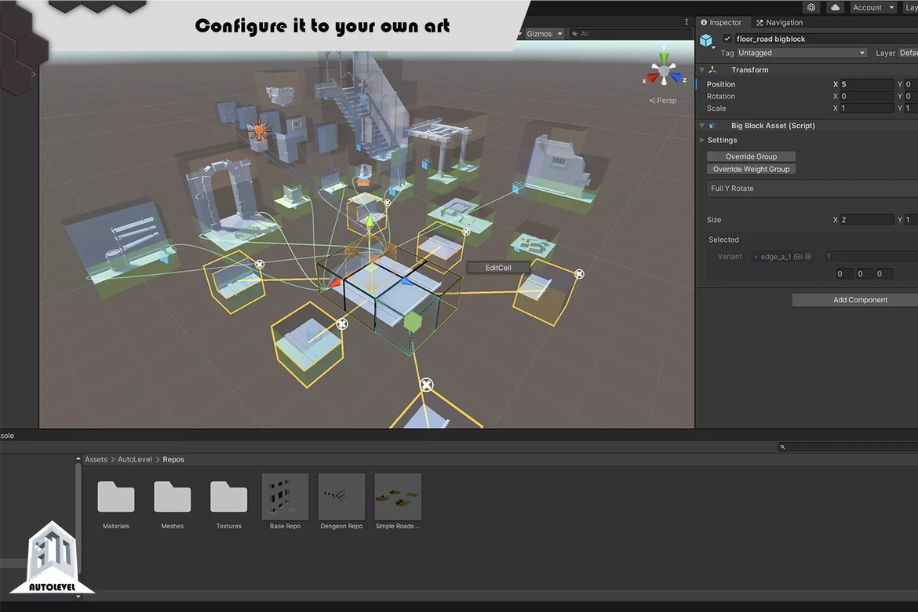
\includegraphics[width=1\linewidth]{content/pictures/FirstSteps02.png}
\caption{Level Builder Komponente (Quelle: \cite{alasl_autolevel_nodate})}
\label{fig:repository-generator}
\end{figure}

Allerdings setzt dieses Paket voraus, dass jedes Struktur gebende \ac{3D}-Objekt in seine 1x1x1 Meter große Basis zerlegt wird. Das wäre bei Assets, die über den Asset-Store hinzugenommen wurden, ein viel zu großer Aufwand geworden.

Daher wurde nach einem Generator geschaut, der fertige Strukturelemente wie Boden-Modelle oder Wand-Elemente verwenden kann. \cite{mysticforge_low_nodate} stellt einen Generator bereit, bei dem für verschiedene Abschnitte, wie Links/ Rechts Kurven, zweier oder dreier Kreuzungen oder geraden Stücken, verschiedene Varianten bereitgestellt werden können und der Generator aus diesen eine Spielwelt generiert. Zusätzlich konnten auch angefertigte Räume mit bereitgestellt werden, in welchen im späteren Verlauf die Rätsel eingebaut werden können. Die Elemente, die zwischen diesen Räumen generiert wurden, können so als Verbindungsstücke dienen, durch welcher der Watcher den Player navigieren müsste. Auch dieser Generator benötigt Modelle in einer bestimmten Größen-Norm. Diese ist jedoch im Vergleich zum Generator von \cite{alasl_autolevel_nodate} nicht zu kleinteilig und bezieht sich auf strukturgebende Elemente wie Wände als Ganzes.

\begin{figure}[ht]
\centering
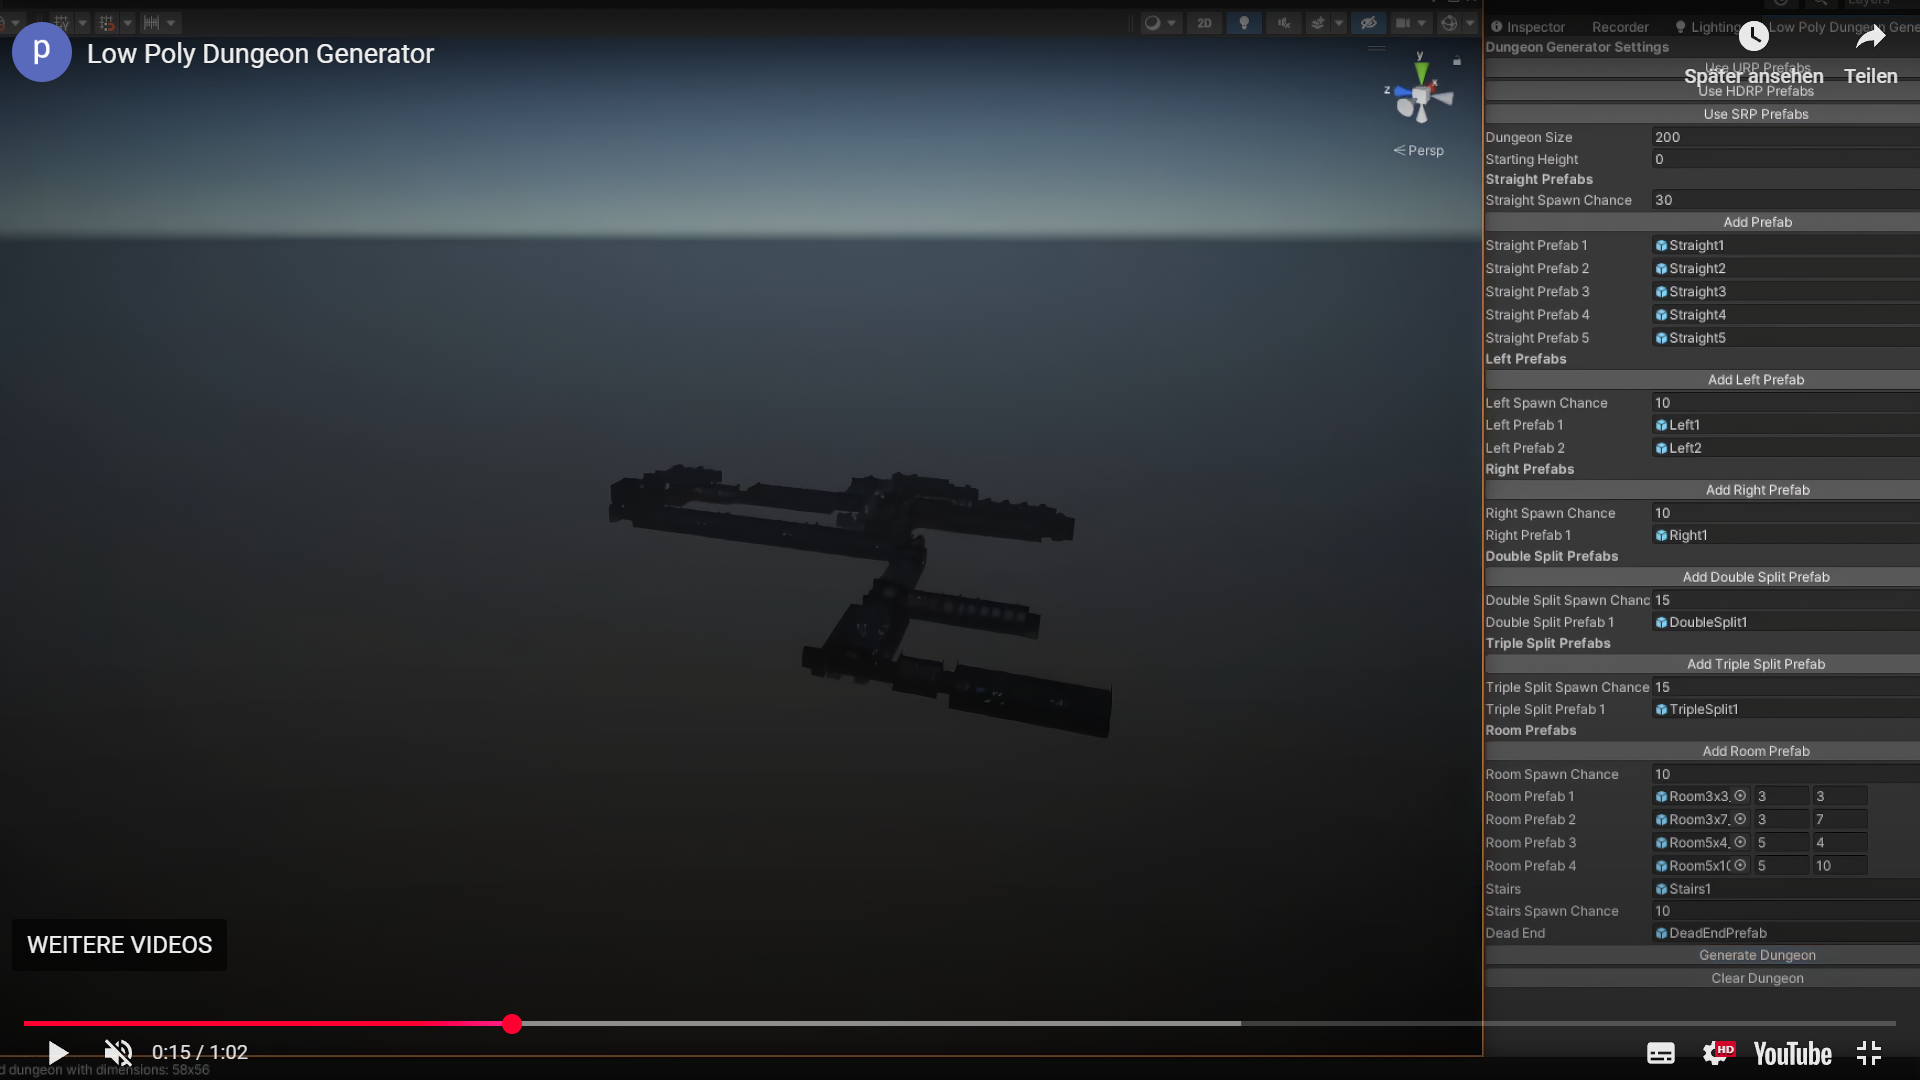
\includegraphics[width=1\linewidth]{content/pictures/FirstSteps03.png}
\caption{Low-Poly Dungeon Generator (Quelle: \cite{past12pm_low_2024})}
\label{fig:dungeon-generator}
\end{figure}

Allerdings werden die verschiedenen Elemente zufällig hintereinander gereiht. Deshalb wurde der Ansatz aus dem vorangegangenem Generator mit eingebaut. So konnte nun bestimmt werden, welche Objekte auf welche Folgen und welche zuvor kommen sollen. Abbildung \ref{fig:athaeck-dungeon-generator} zeigt das Ergebnis aus den in einer in Norm erstellten Strukturelementen (oberes Bild) generierte Wege zwischen den Räumen (unteres Bild). Leider ist es so, dass durch das Zufallsprinzip, zu welcher Wahrscheinlichkeit wann welche Elemente kommen, zu viel Unruhe entsteht und das Ergebnis so für den Anwendungszweck nicht nutzbar ist.

\begin{figure}[ht]
\centering
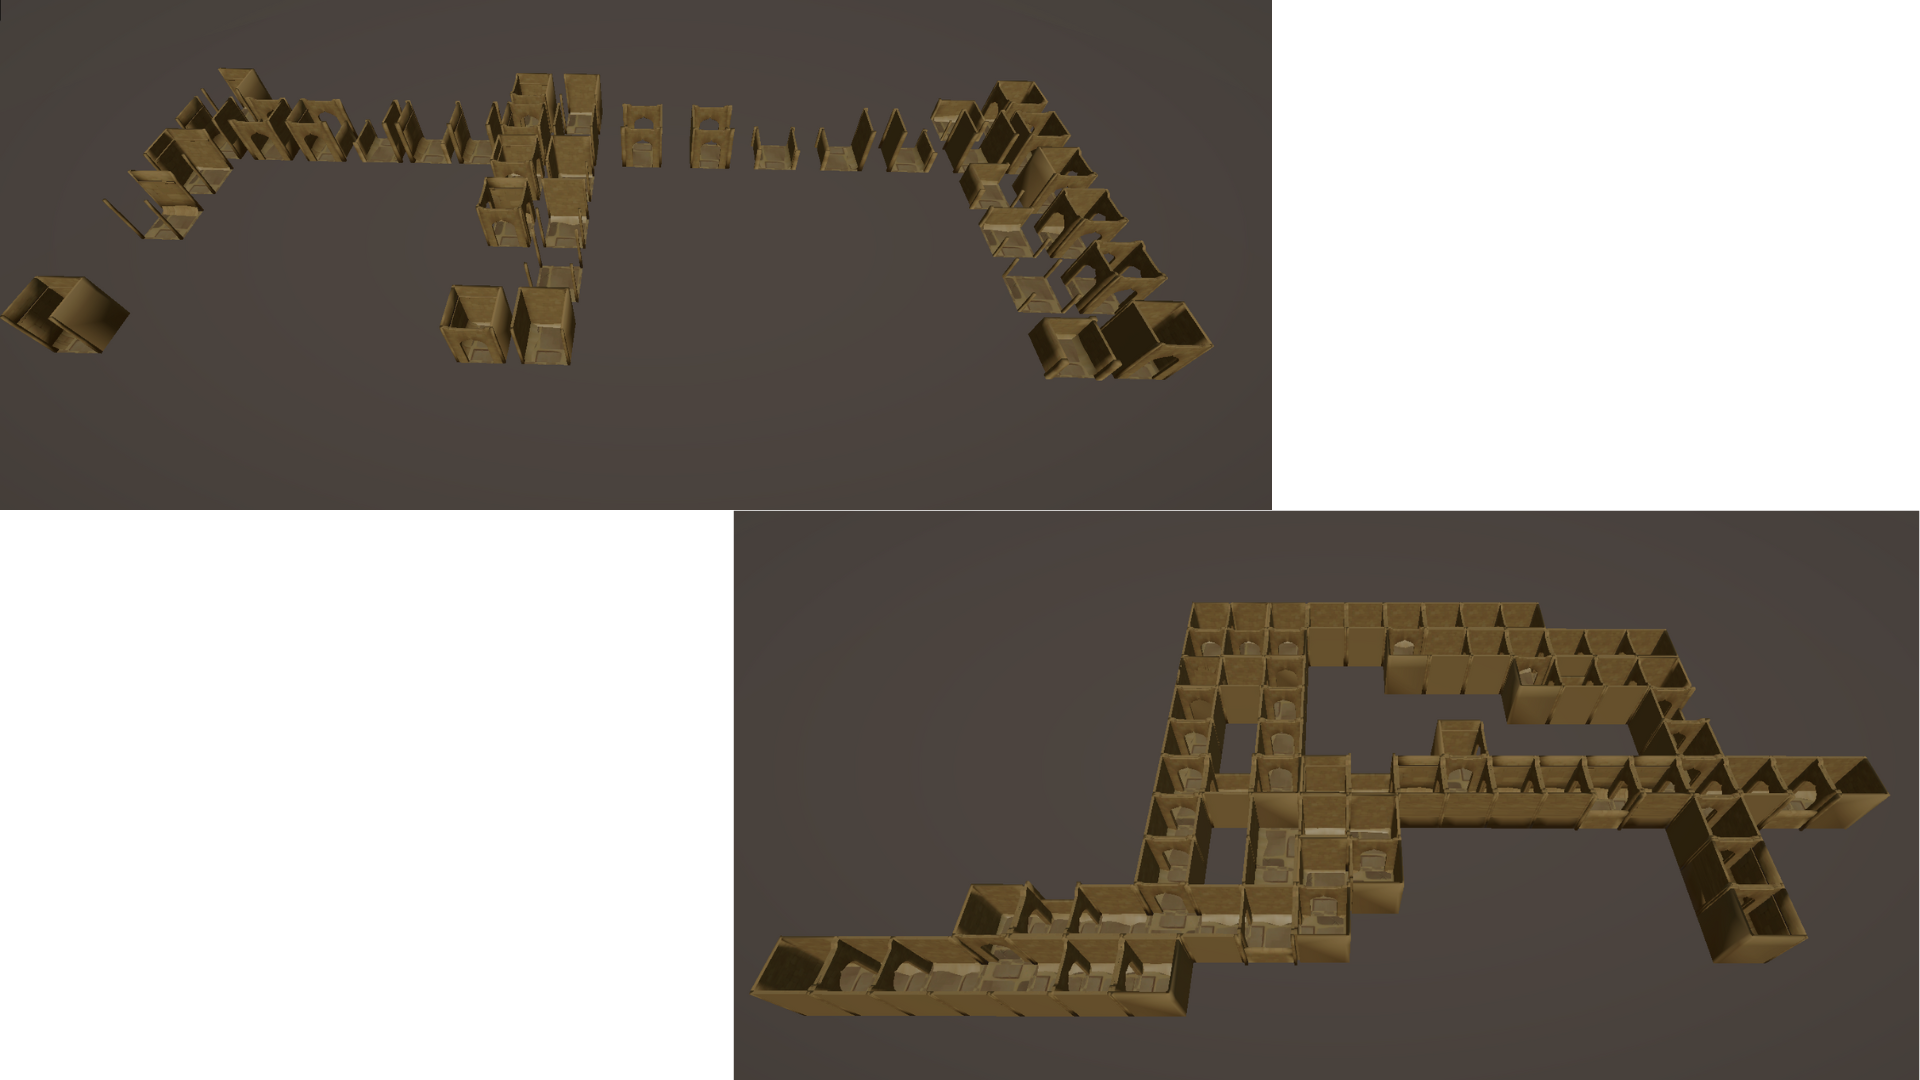
\includegraphics[width=1\linewidth]{content/pictures/FirstSteps06.png}
\caption{athaeck Dungeon Generator (Quelle: eigene Darstellung)}
\label{fig:athaeck-dungeon-generator}
\end{figure}

Jedoch hatte dieser nicht weitergeführte Ansatz auch ein positives Ergebnis. Da die einzelnen Elemente der Strukturelemente in einer bestimmten selbst definierten Norm angepasst werden mussten, konnte im weitere Verlauf das Leveldesign mit diesen Maßstäben die weiteren hinzugenommenen Assets anpassen und verwendet werden.

\subsection{Physik-System von Unity}\label{sec:unity-physics-system}
Die Kern-Mechanik des Lösens von Hindernissen in diesem Prototyp ist das Platzieren von Gegenständen an bestimmte Stellen. Zu einem Teil werden die Platzierungen der Objekte über das Physik-System von Unity überprüft. Jeder platzierte Gegenstand besitzt einen Collider, der auf Kollisionen mit anderen Collidern, wie dem des Player-Avatars reagiert. Wie in den Beispielen der \say{QuestSolver} (vgl. Abschnitt \nameref{sec:quest-system}) oder \say{PathActivator} (vgl. Abschnitt \nameref{sec:path-system}) reagieren nun diese Komponenten auf die Collider der Gegenstände, die innerhalb der eigenen Collider platziert werden (vgl. Abbildung \ref{fig:collision-sketch}). 

% [TODO: Zur veranschaulichung eine Zeichnung eimbauen?]
\begin{figure}[ht]
\centering
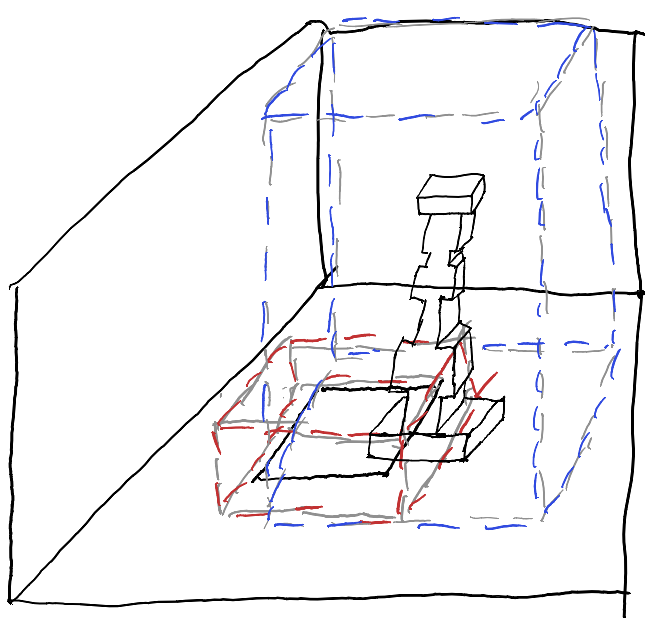
\includegraphics[width=.6\linewidth]{content/pictures/CollisionSketch.png}
\caption{Kollision zweier Collider in dem Raum, bei dem blau und rot sich kreuzen (Quelle: eigene Darstellung)}
\label{fig:collision-sketch}
\end{figure}


Sobald ein Gegenstand innerhalb eines anderen Colliders platziert wird, errechnet das Physik-System eine Kollision, welche in den gehandhabten Klassen nun empfangen werden kann. Das \say{Script lifecycle flowchart} von Unity in \cite{technologies_unity_nodate} zeigt dies anschaulich. Nachdem ein neuer Knoten in die Spielwelt instanziiert wurde, beginnt zunächst die Initialisierung der enthaltenen Skripte. Anschließend erfolgt die Errechnung des Physik-Systems, ehe es weiter über Input-Events und die Spiellogik geht.

Jedoch gab es Probleme beim Entfernen der einzelnen Objekte aus den genannten Zielradien der Collider. Der Lebenszyklus von Unity errechnet, nachdem ein Gegenstand entfernt wurde, keine physikalischen Veränderungen des entfernten Objekts (in der Abbildung nach \say{OnApplicationQuit} zu sehen). Für das Lösungssystem der Hindernisse und der Aktivierung oder Deaktivierung von bestimmten Pfaden ist dies ein Problem.

Aus diesem Grund wurde eine Basisklasse geschrieben, die an den zur Laufzeit hinzugefügten und entfernten Objekten liegt. Von ihr aus sollen nun Kollisionen ausgeführt werden. In der Vergangenheit wurde jeweils an den Objekten, die die Kollisionen empfangen, diese behandelt. Zum Teil bleibt dieses Prinzip erhalten, nur ist diesmal der Verursacher auch derjenige, der zur Laufzeit entfernt wird.

\begin{figure}[ht]
\centering
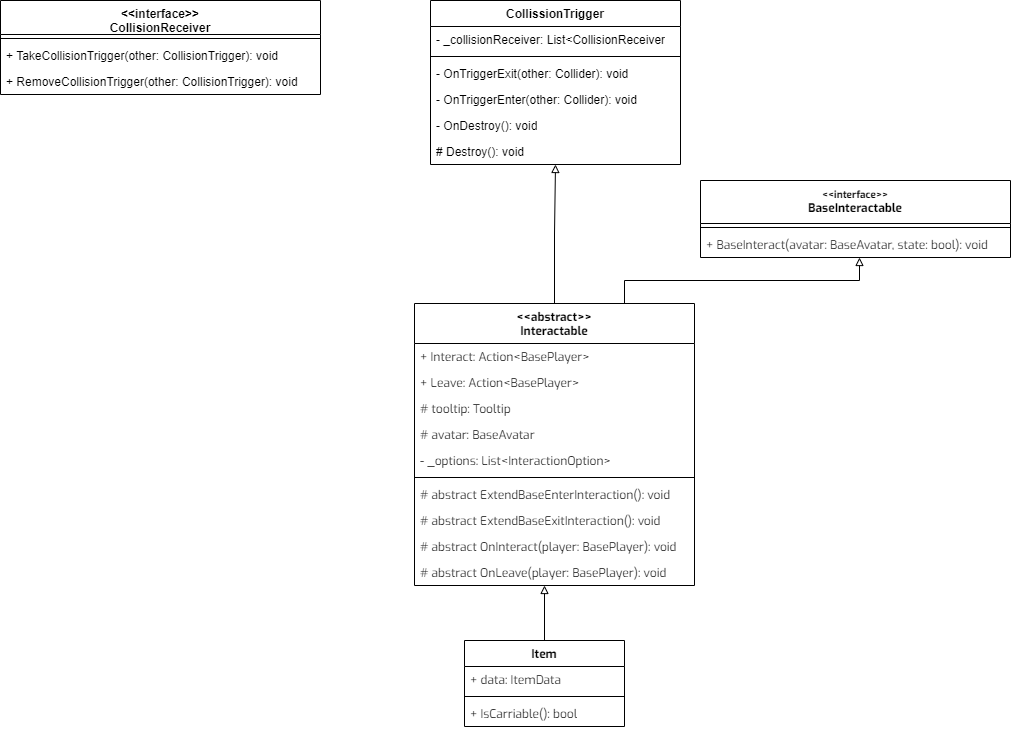
\includegraphics[width=1\linewidth]{content/pictures/CollisionSystem.drawio.png}
\caption{Neue Herangehensweise an Kollisionen (Quelle: eigene Darstellung)}
\label{fig:new-collision-system}
\end{figure}

Abbildung \ref{fig:new-collision-system} zeigt die neue Klasse des \say{Verursachers} von Kollisionen (in letzter Vererbungs-Stufe das \say{Item}-Skript, welches am Gegenstandobjekt liegt, welches platziert wird) und das Empfänger-Interface, das nun wie in Abbildung \ref{fig:new-collision-system-in-quests} von der \say{BasePlaceableActivator} Basis-Klasse vererbt wird. 

\begin{figure}[ht]
\centering
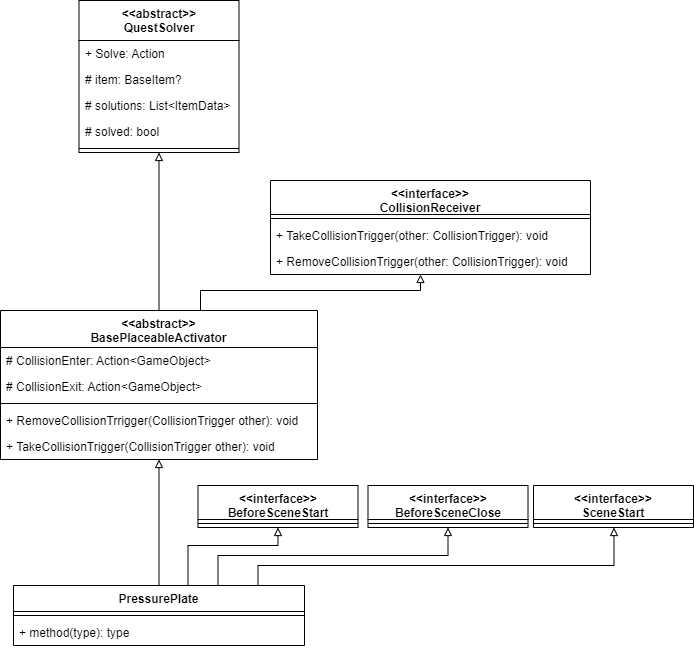
\includegraphics[width=0.8\linewidth]{content/pictures/Quest-Extension.drawio.png}
\caption{Kollisions-Empfänger im Quest-System (Quelle: eigene Darstellung)}
\label{fig:new-collision-system-in-quests}
\end{figure}

\subsection{Platzieren von Gegenständen außerhalb der Spielwelt}\label{sec:difficulties-placement}
Wie bereits erwähnt, besitzen der Player und der Watcher zum Teil unterschiedliche Ansichten der Räume. Am Beispiel des Sicherheitsraumes wird das folgende Problem, das das Platzieren von Gegenständen mit sich führen kann, vorgestellt. 

Im Sicherheitsraum befindet sich der Player innerhalb des Gebäudes, wohingegen der Watcher zusätzlich einen kleinen Außenbereich sieht, auf den er einen gefundenen Stromgenerator platzieren muss. Da sich für den Watcher ein Bereich geöffnet hat, kann er auf diesen den Generator ohne Probleme platzieren. Da jedoch alle in der Session platzierten Gegenstände sowohl beim Watcher als auch beim Player platziert werden, stößt dies auf ein Problem. Der Player darf keine Gegenstände sehen, welche in nicht aktiven Bereichen liegen. 

Aus diesem Grund wurde für jeden Bereich Collider in die Spielwelt platziert, die dafür verantwortlich sind, Gegenstände zu aktivieren oder deaktivieren, je nachdem, ob der Bereich aktiv oder inaktiv ist. Das umgeänderte System aus dem vorangegangenen Kapitel \nameref{sec:unity-physics-system} und die Klasse \say{PathCollider} aus dem Kapitel \nameref{sec:path-system} spielen hier dabei zusammen und ermöglichen es, dass sowohl Player als auch Watcher keine \say{falschen} Objekte außerhalb der aktiven Weltgebiete sehen können.

Jedoch fielen in der Evaluation der Anwendungen Grenzfälle auf, die im Kapitel \nameref{sec:prospect} weiter behandelt werden.



% erste Ansätze im Levelbuilding erwähnen

% hier kommt das placing also die positionen in der spielwelt

% dann drauf bezogen das mit den slots, dass die ne position haben später auch fürs setzen wichtig
% das mit den collidern, was man auch anders umsetzen kann noch, das noch erwähnen






% bei umsetzung müssen die 3d und ar anwendung vorgestellt werden vom watcher
% hier muss ein bezg auf das paper mit den steuerungen für touch erwähnt werden


% die anwendung vom playewr

\section{Probleme in der Umsetzung}
Für die Evaluation ist geplant gewesen, dass die Anwendung des Watchers über eine \ac{AR}-Integration verfügt. Ein Kernelement einer funktionierenden \ac{AR}-Anwendung ist das Platzieren des entsprechenden \ac{3D}-Objektes in den virtuellen Raum, der durch die Sicht des Smartphones aussieht, als wäre er im echten Raum platziert. Damit das Platzieren des Weltobjektes der Anwendung des Watchers auch gut verankert ist, wurde das \say{Place detection}-Modul der \ac{AR}Foundation verwendet. Zusätzlich wurden auf der ausgewählten Plane ein \ac{AR}Anchor platziert, welcher mitHilfe des Anchor-Managers eine zuverlässigeres Platzieren \ac{AR} gewährleisten soll.

Das Ergebnis, das dabei heraus kam, war, dass sich die platzierte Spielwelt in einem bestimmten Abstand zur Kamera immer mitbewegt hat. Zusehen ist dies ebenfalls in diesem Unity-Forum im vorletzten Beitrag von Howard258 \cite{noauthor_unity_2025}. Es wurden einige Lösungsversuche, wie das Umstellen der Zuordnung in der Anchor und Plane Platzierung, oder das Umstellen der Weltknoten, versucht. Jeder neue Ansatz brachte leider keine Lösung für das Platzierungsproblem. In einem weiteren Forum (vgl. \cite{noauthor_ar_2023}) wurde gezeigt, dass die genutzte Version der \ac{AR}Foundation und der Unity-Editor Version ein Grund für die deffekte \ac{AR}-Platzierung ist. Dieser Lösungsweg wurde aus zeitlichen Gründen nicht mehr umgesetzt, da eine Versions-Änderung des Editors und seine enthaltenen Assets auch zu weiteren Problemen führen könnten. 

Ebenfalls wurde auch keine weitere Platzierungsmethode wie das \say{Image tracking} verwendet, da sich der Watcher frei in seiner physischen Welt bewegen soll und die Gefahr besteht, dass das Vergleichsbild nicht meehr gesehen wird und der Spieler keine Spielwelt vor sich sieht.
% AR

% Gerätefindung im selben Netzwerk -> eher Herausforderungen in der Evaluation